
\documentclass[12pt]{article}

\usepackage[bottom=3cm]{geometry}
\usepackage{p4doc}
\usepackage{fleqn}
\usepackage{fancyvrb}
\usepackage{graphicx}
\usepackage{tabularx}
\usepackage{soul}
\usepackage{float}
\usepackage{underscore}
\usepackage[table]{xcolor}

\usepackage[parfill]{parskip}

\usepackage{silence}
\WarningFilter{Fancyhdr}{\headheight is too small}
\WarningFilter{latex}{Overfull \hbox}


%%not_a_keyword auto
%%not_a_keyword default

%%not_a_keyword expression_local_variables

%%not_a_keyword ternary
%%not_a_keyword exact
%%not_a_keyword lpm

%%not_a_keyword length

%%not_a_keyword type

%%not_a_keyword reads
%%not_a_keyword actions
%%not_a_keyword min_size
%%not_a_keyword max_size
%%not_a_keyword size
%%not_a_keyword modifier
%%not_a_keyword support_timeout


\lstdefinestyle{BNFstyle}{
    language=BNF,%
    frame=single,%
    backgroundcolor=\color{bnfgreen},%
    morekeywords={const_value, unsigned_value, bool_value, binary_value, decimal_value, hexadecimal_value, binary_base, hexadecimal_base, binary_digit, decimal_digit, hexadecimal_digit, width_spec, field_value, type_spec, data_type, data_type_qualifier, typedef_declaration, object_ref, general_expr, bool_expr, arith_expr, bin_op, un_op, bool_op, rel_op, header_type_declaration, header_dec_body, field_dec, length_bin_op, length_exp, header_instance_declaration, metadata_initializer, local_variable_declaration, struct_type_declaration, struct_member, struct_instance_declaration, header_ref, index, field_ref, field_list_declaration, field_list_entry, parser_function_declaration, parser_function_body, parser_body_call, extract_statement, set_statement, metadata_expr, parser_subroutine_call, return_statement, return_value_type, case_entry, value_list, case_return_value_type, value_or_masked, select_exp, field_or_data_ref, parser_exception_declaration, return_or_drop, return_to_control, action_function_declaration, action_header, param_list, param, param_qualifier, action_statement, arg_list, table_declaration, table_attribute, field_match, possibly_masked_ref, field_match_type, control_function_declaration, control_block, control_statement, apply_call, apply_and_select_block, case_list, action_case, action_or_default, hit_miss_case, hit_or_miss, if_else_statement, else_block, whitebox_type_declaration, whitebox_instance_declaration, whitebox_prototype_declaration, type_variable_list, blackbox_type_declaration, member_declaration, method_declaration, attribute_declaration, identifier_list, attribute_type, blackbox_instance_declaration, blackbox_attribute_binding, blackbox_method_call, p4_program, p4_declaration}%
}

\lstdefinestyle{P4style}{
    language=C,%
    frame=single,%
    backgroundcolor=\color{codeblue},%
    keywords={accept, action, and, apply, attribute, bit, blackbox, blackbox_type, block, control, current, else, expression, extract, false, field_list, fields, header, header_array, header_type, hit, if, in, inout, int, last, local, mask, max, metadata, method, min, miss, next, not, optional, or, out, parser, parser_drop, parser_exception, range, return, saturating, select, set_metadata, signed, string, struct, struct_type, table, true, typedef, valid, value, varbit, void, whitebox, whitebox_type},%
    basicstyle=\ttfamily,%
    aboveskip=3mm,%
    belowskip=3mm,%
    fontadjust=true,%
    keepspaces=true,%
    keywordstyle=\bfseries,%
    captionpos=b,%
    framerule=0.3pt,%
    firstnumber=0,%
    numbersep=1.5mm,%
    numberstyle=\tiny,%
}

\ifpdf
    \pdfinfo {
        /Author   (The P4 Language Consortium)
        /Title    (The P4 Language Specification, v 1.1.0 rc1)
        /Keywords (P4)
        /Subject  ()
        /Creator  (TeX)
        /Producer (PDFLaTeX)
    }
\fi

\begin{document}
\vspace{2cm}

%\title{\sffamily\bfseries\huge The P4 Language Specification\\ \vspace{3mm} \Large Version 1.0.2}
\centerline{\sffamily\bfseries\huge The P4 Language Specification}
\vspace{3mm}
\centerline{\sffamily\Large Version 1.1.0 rc1}
\vspace{3mm}
\centerline{\sffamily\large August 12, 2015}
\vspace{8mm}
\centerline{\sffamily\large The P4 Language Consortium}

\date{August 12, 2015}
\thispagestyle{firstpagestyle}
%\maketitle

\SECTION{Introduction}{intro}

P4 is a declarative language for expressing how packets are processed by the 
pipeline of a network forwarding element such as a switch, NIC, router or 
network function appliance. P4 itself is protocol independent but allows for
the expression of existing and future forwarding plane protocols. 

It is based upon a set of common abstractions for packet processing including a
state machine \textit{parser} to describe the order and connection between
packet headers and a set of \matchaction tables arranged into an imperatively
executed program. The parser identifies the headers present in each incoming
packet. Each \matchaction table performs a lookup on a subset of header fields
and applies the actions corresponding to the first match within each table.

\begin{itemize}
\item
\textit{Header definitions:} the format (the set of fields and their
sizes) of each header within a packet.
\item
\textit{Parse graphs:} the permitted header sequences within packets.
\item
\textit{Table definitions:} the type of lookup to perform, the input
fields to use, the actions that may be applied, and the dimensions of
each table.
\item
\textit{Action definitions:} compound actions composed from a set of
primitive actions.
\item
\textit{Pipeline layout and control flow:} the layout of tables within
the pipeline and the packet flow through the pipeline.
\end{itemize}

P4 addresses the configuration of a forwarding element. Once configured, tables 
may be populated and packet processing takes place. These post-configuration 
operations are referred to as "run time" in this document. This does not preclude 
updating a forwarding element's configuration while it is running.

A machine that can run a P4 program is called \textit{target}. Each target
conforms to a \textit{Target Architecture}, specified partially as a library of
P4 code and partially as a set of instructive non-P4 documents, which describes
the programmable regions of the target and how those regions connect to each
other. These regions include things like packet parsers, and pipelines of tables
and actions.

\SUBSECTION{Target Architectures}{archs}

While P4 provides a standard language for describing the logic within
programmable portions of a forwarding element, what programmable portions are
actually available and the data flow between those portions will likely vary
from target to target.

For example, one target may consist of a parser, ingress \matchaction pipeline
and egress \matchaction pipeline, connected in sequence. Another target may
consist of several parser-pipeline pairs, which the packet may flow through
in any order by setting the appropriate control signals. While P4 can address
the contents of each of the above regions, it does not attempt to standardize
any one architectural model. Instead, it provides the facilities for target
providers and standards bodies to define multiple such architectures.

A P4 \textit{Target Architecture} is the complete specification of a P4
target's programmable resources and the way those resources are connected. The
architecture consists of both P4 code and an external written specification.

\SUBSUBSECTION{Target Architecture Structure}{archsstruct}

The P4 portion of a target architecture provides \textit{prototypes} for the
programmable portions of the chip. These prototypes specify the special control
signals, or \textit{intrinsic metadata}, that are available to each portion of
the target. This intrinsic metadata forms an interface between the region of
code in question and the external non-P4-programmable environment. For instance,
a region of code may receive intrinsic metadata reporting a packet's ingress
port and length, and may write intrinsic metadata controlling the packet's
egress port and queue priority.

The P4 portion of the architecture may also provide definitions of primitive
actions (Section~\ref{sec:actions}) and blackbox object types
(Section~\ref{sec:bboxes}), which represent the fundamental processing
capabilities of the target. Examples of these include arithmetic functions and
checksum generators.

The external written specification clarifies the meaning of the definitions
in the P4 portion of the architecture and explains how they fit together. It
is mostly human language documentation and visual diagrams to show the flow of
data between programmable blocks, though it may also contain pseudocode to
rigorously specify the behavior of logic not expressible in P4.

For an example of an architecture definition, see the Simple Switch Architecture
in Section~\ref{sec:simplearch}. The code examples used inline in this document
assume the use of this architecture.

\SUBSUBSECTION{Target Architecture Selection}{archsselect}

A program's target architecture is selected by including that architecture's P4
library in the source code and writing structures that conform to the prototypes
it specifies.

No one architecture is mandated by the P4 spec and a given physical target may 
support multiple architectures. Some architectures may be written by a target
provider and highly specialized to their underlying machine, while others may
be standardized and intentionally abstracted to allow greater portability and
ease-of-use.

Regardless, all P4 programs written for a given architecture are portable across
all targets that faithfully implement said architecture (assuming that enough
resources are available). P4 conformance of a target is defined as follows: if a
specific target supports a given target architecture, a program written in that
architecture and executed on the target should provide the exact same behavior
as the same program executed  on an abstract machine with infinite resources.

In general, P4 programs are not expected to be portable across different
architectures. For example, executing a P4 program that controls packet
broadcast by writing special intrinsic metadata will not work on a target that
provides no such intrinsic metadata.

Further, particular targets may not support fully some P4 language constructs
(for example, some targets may not support the features necessary for IPv4
options processing or arbitrary-length stacked protocol headers). Ideally the
restrictions on the P4 language imposed by a specific target should be clearly
documented by the target architecutre; at the very least, restrictions have to
be conveyed to P4 programmers using clear compiler error messages when
attempting to compile programs that use unsupported features.

\SUBSECTION{The mTag Example}{mtag}

The original P4 paper [1] includes an example called mTag. We use this example 
throughout this specification as a means of explaining the basic language 
features as they are presented. Complete source for this example, including 
sample run time APIs, is available at the P4 web site [2].

We give an overview of the mTag example here.  Quoting from the original paper:

\begin{quote}
Consider an example L2 network deployment with top-of-rack (ToR) switches 
at the edge connected by a two-tier core. We will assume the number of end-hosts 
is growing and the core L2 tables are overflowing. . . .  P4 lets us express a 
custom solution with minimal changes to the network architecture. . . . The routes 
through the core are encoded by a 32-bit tag composed of four single-byte 
fields.  The 32-bit tag can carry a "source route".... Each core switch need 
only examine one byte of the tag and switch on that information. [1]
\end{quote}

Two P4 programs are defined for this example: One for edge switches (called 
"ToR" above) and one for aggregation switches (called "core switches" above). 
These two programs share definitions for packet headers, the parser and actions.
Both programs use the Simple Switch Architecture described in section
\ref{sec:simplearch}.

\SUBSECTION{Specification Conventions}{conventions}

This document represents P4 grammatical constructs using BNF with the
following conventions:

\begin{itemize}
\item
The BNF is presented in green boxes.
\item
Non-terminal nodes are indicated with \textbf{bold}.
\item
A node with a name ending in \texttt{_name} is implicitly a string whose first character 
is a letter (not a digit).
\item
Nodes followed by \texttt{+} indicate one or more instances.
\item
Nodes followed by \texttt{*} indicate zero or more instances.
\item
A vertical bar, \texttt{|}, separates options from which exactly one must be selected.
\item
Square brackets, \texttt{[]}, are used to group nodes. A group is optional unless 
it is followed by \texttt{+}. A group may be followed by * indicating zero or more 
instances of the group.
\item
Symbols with special significance (e.g., \texttt{[ ] * + |}) may be used as terminal 
nodes by enclosing them in quotes: for example "\texttt{*}".
\item
Symbols other than those listed above are literals. Examples include curly 
braces, colon, semi-colon, parentheses, and comma.
\item
If a rule does not fit on one line, a new line immediately follows \texttt{::=} and 
the description ends with a blank line.
\item
Example P4 code appears in blue boxes
\item
Example code in a language other than P4 appears in beige boxes
\end{itemize}

\SECTION{Structure of the P4 Language}{structure}

\SUBSECTION{Abstractions}{p4abstractions}

P4 provides the following top-level abstractions: 

\begin{itemize}
\item
\textit{Headers:}
\begin{itemize}
\item
\textit{Header types:} A specification of fields within a header.
\item
\textit{Header instances:} A specific instance of a packet header or metadata.
\end{itemize}
\item
\textit{Parser state function:} Defines how headers are identified
within a packet.
\item
\textit{Action function:} A composition of primitive actions that are to be applied 
together.
\item
\textit{Table instance:} Specified by the fields to match and the permitted actions.
\item
\textit{Control flow function:} Imperative description of the table application
order. 
\item
\textit{Blackboxes:}
\begin{itemize}
\item
\textit{Blackbox types:} An object type provided by a standard library 
or target provider which can perform functionality not otherwise expressible
in P4.
\item
\textit{Blackbox instances:} A specific instance of a blackbox type.
\end{itemize}
\item
\textit{Whiteboxes:}
\begin{itemize}
\item
\textit{Whitebox types:} An excerpt of P4 code that forms a "code template"
which can be instantiated multiple times.
\item
\textit{Whitebox instances:} A specific instance of a whitebox type.
\end{itemize}
\end{itemize}


\SUBSECTION{Value Specifications}{valuespec}

P4 supports generic and bit-width specific values. These are unified through
the following representation.

%%bnf
\begin{lstlisting}[style=BNFstyle]
const_value ::=
    bool_value |
    [ "+" | - ] [ width_spec ] unsigned_value

unsigned_value ::= 
    binary_value | 
    decimal_value | 
    hexadecimal_value

bool_value ::= true | false
binary_value ::=  binary_base binary_digit+
decimal_value ::= decimal_digit+
hexadecimal_value ::= hexadecimal_base hexadecimal_digit+

binary_base ::= 0b | 0B
hexadecimal_base ::= 0x | 0X

binary_digit ::= _ | 0 | 1
decimal_digit ::= binary_digit | 2 | 3 | 4 | 5 | 6 | 7 | 8 | 9
hexadecimal_digit ::= 
    decimal_digit | a | A | b | B | c | C | d | D | e | E | f | F

width_spec ::= decimal_digit+ :
field_value ::= const_value
\end{lstlisting}
%%endbnf

Note that constants always start with a digit to distinguish them from other 
identifiers.

The node \texttt{const_value} may be read as 'constant value'. The node
\texttt{field_value} is used in this specification to emphasize that the width
of the representation may be relevant; otherwise it is a synonym for
\texttt{const_value}.

Whitespace terminates a constant specification.

Underscores are permitted in values to add clarity by grouping digits; they are
ignored otherwise. Examples include: \texttt{78_256_803} (replacing commas in
decimal representation) or \texttt{0b1101_1110_0101} (grouping bits into nibbles
or bytes in binary representation).

Optionally, the bit-width of the value may be specified as indicated by
\texttt{width_spec}. If no width precedes the value, or a width of 0 is used,
then the width is inferred. For positive values the inferred width is the
smallest number of bits required to contain the value. For negative values the
inferred width is one more than the smallest number of bits required to contain
the positive value.

Negative numbers are represented in two's complement. See 
Section~\ref{sec:p4casting} regarding conversions and sign extension of field 
values.

Here are some example values.

\begin{table}[H]
\begin{center}
\begin{tabular}{| l | l | l | p{.5\textwidth} |} \hline
\textbf{Notation} &
\textbf{Decimal Value} & 
\textbf{Bit Width} &
\textbf{Notes} \\ \hline
\texttt{42} &
42 &
6 &
Default base is decimal \\ \hline
\texttt{16w42} &
42 &
16 &
The same value, but explicitly given a width of 16 bits. \\ \hline
\texttt{0b101010} &
42 &
6 &
Binary representation of same with implicit width \\ \hline
\texttt{0w0x2a} &
42 &
6 &
The width '0' is the same as not specifying a width meaning the width is inferred from the value.   \\ \hline
\texttt{12w0x100} &
256 &
12 &
Example of bit width and hexadecimal base indication. \\ \hline
\texttt{7w0b1} &
1 &
7 &
Binary value specified with explicit width \\ \hline
\texttt{-0B101} &
-5 &
4 &
The negative is not applied until the rest of the value is evaluated. \\ \hline
\end{tabular}
\end{center}
\caption{Value Representation Examples}
\end{table}

\SUBSECTION{Types and declarations}{p4types}

A P4 program consists of concrete declarations of the abstractions listed in
Section~\ref{sec:p4abstractions}.

Object declarations occur either at the top-level of the program or inside a
whitebox definition; declarations cannot happen conditionally, such as inside
a specific parse state or branch of a control flow. Declarations consist of
a type, as specified in the grammar below, followed by a unique identifier
and an object body. The exact format of the body depends on the object type,
and is described in more detail for each type throughout this document.

The order that objects are declared in does not matter, and objects can
reference other objects that were declared before them in the code.

P4 types generally consist of the kind of abstraction, followed by the specific
type name in the case of headers, blackboxes and whiteboxes:

%%bnf
\begin{lstlisting}[style=BNFstyle]

type_spec ::=
    header [ header_type_name ] |
    metadata [ header_type_name ] |
    struct [ struct_type_name ] |
    blackbox [ blackbox_type_name ] |
    whitebox [ whitebox_type_name ] |
    header_array |
    field_list |
    parser |
    parser_exception |
    action |
    table |
    control |
    data_type

data_type ::=
    bit |
    bit < decimal_digit+ [ , data_type_qualifier ]* > |
    bit < auto > |
    varbit < decimal_digit+ > |
    int | 
    void

data_type_qualifier ::= signed | saturating

typedef_declaration ::=
    typedef type_spec new_type_name ;

\end{lstlisting}
%%endbnf

P4 actions and whiteboxes consist of signatures which look like the typed
parameter lists of traditional programming languages. The types of the
parameters in these signatures must be one of the above.

The \textit{bit} type represents a bitstring of the length specified within
angle brackets (a compile time constant). If the angle brackets are omitted, the
length is implied to be 1. Most of the data processed by P4 is stored in a
bitstring of some sort, cast appropriately when arithmetic must be performed.
They are, by default, unsigned and non-saturating (i.e., addition/subtraction
causing overflow/underflow will wrap). These properties can be changed by adding
type qualifiers inside the type's angle brackets. See
Section~\ref{sec:p4casting} for more information.

The \textit{varbit} type represents a bitstring with a length that is variable
at run time, but \textit{at most} the length specified within angle brackets
(again, a compile time constant). This datatype is used for quickly parsing
through variable length headers and does not currently have utility beyond
that. More functionality may be added for this type in subsequent versions of P4
(such as the ability to read it from a \matchaction pipeline).

The \textit{int} type represents a signed arbitrarily large integer, which is
used for numeric constant parameters and other situations in which a
bitstring-like type is needed but doesn't have a well-defined bit width
apparent from context.

Bitstrings with a width of 0 are used for action and method parameters which are
agnostic to the bit width of the arguments bound to them, but require a finite-
width bitstring all the same. It is an error to use this outside of a parameter
list or blackbox attribute declaration, since it implies a fixed-width bitstring
whose width is inferred at compile-time.

Types which are followed by an optional identifier like \textit{header} and
\textit{struct} can be used in two ways:
\begin{itemize}
\item
    "\texttt{header foo}" refers to a header instance specifically of
    header_type \textit{foo}
\item
    "\texttt{header}" without an identifier refers to any header instance,
    of \textit{any} type.
\end{itemize}

New types may be derived from pre-existing ones using the standard typedef
mechanism.

\SUBSECTION{Type qualifiers and value conversions}{p4casting}

TODO: This section was copied more or less from the public spec, which leaves
this behavior still somewhat ambiguous. Signed and saturating data support in P4
needs more thought put into it.

\SUBSUBSECTION{Arithmetic}{castingarith}

The type qualifiers on a bitstring influence the behavior of arithmetic and
comparison operators in expressions that contain them, as well as any primitives
or blackboxes that implicitly use them for arithmetic. This behavior is as
follows:

\begin{lstlisting}[language=C,frame=single,backgroundcolor=\color{nonp4orange},escapechar=!]
tmp = data + value
if (data.saturating && tmp < data.min)
    result = data.min
else if (data.saturating && tmp > data.max)
    result = data.max
else
    result = tmp % !$2^{data.width}$!
\end{lstlisting}

where:

\begin{itemize}
\item
\texttt{data.saturating}: boolean value indicating that the bitstring is
saturating.
\item
\texttt{data.min}: minimum allowed value determined by the bitstring's bit width
and signedness
\item
\texttt{data.max}: maximum allowed value determined by the bitstring's bit width
and signedness
\item
\texttt{data.width}: bit width of the bitstring
\end{itemize}

\SUBSUBSECTION{Width conversions}{castingwidth}

Values may need to be converted when used in an expression or assigned to a
field instance. The conversion will depend the the source and destination widths
and signedness, and whether the destination is saturating.

A value is signed if it has an explicit minus ("\texttt{-}") preceding its
representation or its was declared with a type containing the 'signed'
qualifier. Otherwise it is unsigned.

The rules for conversion are as follows:

\begin{itemize}
\item
If the source and destinations have the same width, the binary value
of the source is used, but the interpretation may change if the
signedness is different.
\begin{itemize}
\item
Example: source is unsigned, 7 bits with a value of 127 and the dest
is signed, 7 bits, the result will be interpreted as -1.
\end{itemize}
\item
If the source width is less than the destination width, the source is
extended based on its own signedness.
\begin{itemize}
\item
Example: Source is signed, 7:0b1111111 and dest is 8 bits; the result is 
8:0b11111111.
\item
Example: Source is unsigned 4:0b1100 and dest is 8 bits; the result is
8:0b00001100.
\end{itemize}
\item
If the source width is greater than the destination width, the result
depends on whether the destination is saturating.  The effect should
be the same as adding the value represented by the source to the
destination when the destination is 0.
\begin{itemize}
\item
Example: Source is signed, and negative, destination is
saturating. the result is 0.
\item
Example: Source is unsigned, has value 17 and the destination is 4
bits, unsigned and saturating; the result is 15 as that is the
saturated value of the destination.
\item
Example: As above, but the destination is not saturating; the result is 1 
as the destination would wrap above 15. This is equivalent to truncating the 
source.
\end{itemize}
\end{itemize}

For expressions, the value with largest bit width is identified and
all other values are converted to this width according to their own
signedness.  The expression is then evaluated and the result is
converted as necessary according to its use.

\SUBSECTION{References}{p4refs}

Concrete instances of the above types are referenced using dotted notation,
where objects that form new scopes may enclose other objects (such as a field
inside a header instance, or a header instance inside a struct). P4 is
lexically scoped.

%%bnf
\begin{lstlisting}[style=BNFstyle]
object_ref ::=
    object_name |
    header_ref |
    field_ref |
    object_name . object_ref
\end{lstlisting}
%%endbnf

The terminal \textit{object_name} refers to any named object within the scope
of a given line of code, while header and field references are handled
specially as described in Section~\ref{sec:headerreferences}.

\SUBSECTION{Expressions}{p4expressions}

Various language constructs can contain expressions built out of these object
references.

%%bnf
\begin{lstlisting}[style=BNFstyle]

general_expr ::= 
    bool_expr | arith_expr | object_ref

bool_expr ::=
    valid ( object_ref ) | bool_expr bool_op bool_expr |
    not bool_expr | ( bool_expr ) | arith_expr rel_op arith_expr |
    bool_value

arith_expr ::=
    object_ref | value | 
    max ( arith_expr , arith_expr ) | min ( arith_expr , arith_expr ) |
    ( arith_expr ) | arith_expr bin_op arith_expr | un_op arith_expr

bin_op ::= "+" | "*" | - | << | >> | & | "|" | ^
un_op ::= ~ | -
bool_op ::= or | and
rel_op ::= > | >= | == | <= | < | !=

\end{lstlisting}
%%endbnf

Operator precedence and associativity follows C programming conventions.

The \textit{min} and \textit{max} functions return whatever is the smaller or
larger of their two arguments, respectively, or the first argument if the two 
compare equally.

\SECTION{Headers and Fields}{hdrs}

\SUBSECTION{Header Type Declarations}{headertypes}

Header types describe the layout of fields and provide names for referencing 
information. Header types are used to declare header and metadata instances. 
These are discussed in the next section.

Header types are specified declaratively according to the following BNF:

%%bnf
\begin{lstlisting}[style=BNFstyle]
header_type_declaration ::= 
   header_type header_type_name { header_dec_body }

header_dec_body ::=
    fields { field_dec * }
    [ length : length_exp ; ]

field_dec ::= type_spec field_name ;
length_bin_op ::= "+" | - | "*" | << | >>
length_exp ::=
    const_value |
    field_name |
    length_exp length_bin_op length_exp |
    ( length_exp )

\end{lstlisting}
%%endbnf

Header types are defined with the following conventions.
\begin{itemize}
\item
Header types must have a \texttt{fields} attribute. 
\begin{itemize}
\item
The list of individual fields is ordered.
\item
Fields must be either of type \textit{bit} or \textit{varbit}.
\item
The bit offset of a field from the start of the header is determined by the 
sum of the widths of the fields preceding it in the list.
\item
Bytes are ordered sequentially (from the packet ordering).
\item
Bits are ordered within bytes by most-significant-bit first.  Thus, if the 
first field listed in a header has a bit width of 1, it is the high order 
bit of the first byte in that header.
\item
All bits in the header must be allocated to some field.
\item
One field at most within a header type may be of type \textit{varbit}, which 
indicates it is of variable length.
\end{itemize}

\item
If all fields are fixed width (no fields of type \textit{varbit}) then the header is 
said to be of \textit{fixed length}. Otherwise it is of \textit{variable length}.
\item
The \texttt{length} attribute specifies an expression whose evaluation gives
the length  of the header in \textit{bytes} for variable length headers. 
\begin{itemize}
\item
It must be present if the header has variable length (some field has type  
\textit{varbit}).
\item
A compiler warning must be generated if it is present for a fixed length header.
\item
Fields referenced in the length attribute must be located before the variable 
length field.
\end{itemize}
\item
If, at run time, the calculated length results in more data extracted to
the \textit{varbit} than its declared maximum length a parser exception is
triggered. See Section~\ref{sec:parserexceptions}.

\item
Operator precedence and associativity follows C programming conventions.
\end{itemize}

An example declaration for a VLAN header (802.1Q) is:

%%code
\begin{lstlisting}[style=P4style]
header_type vlan_t {
    fields {
        bit<3>  pcp;
        bit     cfi;
        bit<12> vid;
        bit<16> ethertype;
    }
}
\end{lstlisting}
%%endcode

Metadata header types are declared with the same syntax.

%%code
\begin{lstlisting}[style=P4style]
header_type packet_metadata_t {
    fields {
        bit<16> ingress_port; // The port on which the packet arrived.

        bit<16> length;       // The number of bytes in the packet. 
                              // For Ethernet, does not include the CRC. 
                              // Cannot be used if the switch is in
                              // 'cut-through' mode.

        bit<8>  type;         // Represents the type of instance of
                              // the packet: 
                              //   - PACKET_TYPE_NORMAL
                              //   - PACKET_TYPE_INGRESS_CLONE
                              //   - PACKET_TYPE_EGRESS_CLONE
                              //   - PACKET_TYPE_RECIRCULATED
                              // Specific compilers will provide macros
                              // to give the above identifiers the
                              // appropriate values
    }
}
\end{lstlisting}
%%endcode

P4 supports variable-length packet headers via fields of type \textit{varbit}.
The width of such a field is inferred from the total header length (which
is in bytes) as indicated by the \texttt{length} attribute: \texttt{((8 *
length) - sum-of-fixed-width-fields)}. Only one field at most within a header
may specify a field of type \textit{varbit}.

An example of a variable-width header is IPv4 with options:

%%code
\begin{lstlisting}[style=P4style]
header_type ipv4_t {
    fields {
        bit<4> version;
        bit<4> ihl;
        bit<8> diffserv;
        bit<16> totalLen;
        bit<16> identification;
        bit<3> flags;
        bit<13> fragOffset;
        bit<8> ttl;
        bit<8> protocol;
        bit<16> hdrChecksum;
        bit<32> srcAddr;
        bit<32> dstAddr;
        varbit<320> options;
    }
    length : ihl * 4;
}
\end{lstlisting}
%%endcode

This header can be parsed and manipulated the same way fixed-length headers
are, with the exception that there are no language facilities to read or
write data in the \textit{options} field.

\SUBSECTION{Header and Metadata Instances}{headerinstances}

While a header type declaration defines a header \textit{type}, a packet may contain 
multiple instances of a given type.  P4 requires each header instance to 
be declared explicitly prior to being referenced. 

There are two sorts of header instances: packet headers and metadata. Usually, 
packet headers are identified from the packet as it arrives at ingress while 
metadata holds information about the packet that is not normally represented 
by the packet data such as ingress port or a time stamp.  

Most metadata is simply per-packet state used like scratch memory while
processing a packet. However, some metadata may have special significance to
the operation  of the forwarding element. For example, the queuing system may
interpret the value of a particular metadata field when choosing a queue for a
packet. P4 acknowledges these target specific semantics, but does not attempt
to represent them.

Packet headers (declared with the \texttt{header} keyword) and metadata (declared 
with the \texttt{metadata} keyword) differ only in their validity. Packet headers 
maintain a separate valid indication which may be tested explicitly. Metadata 
is always considered to be valid. This is further explained in 
Section~\ref{sec:testing}.  Metadata instances are 
initialized to 0 by default, but initial values may be specified in their 
declaration.

The BNF for header and metadata instances is:

%%bnf
\begin{lstlisting}[style=BNFstyle]
header_instance_declaration ::=
    header header_type_name instance_name ; |
    header header_type_name instance_name "[" const_value "]" ; |
    metadata header_type_name instance_name [ metadata_initializer ] ;

metadata_initializer ::= { [ field_name : field_value ; ] + }

local_variable_declaration ::= local type_spec variable_name;

\end{lstlisting}
%%endbnf


Some notes:

\begin{itemize}
\item
Only packet headers (not metadata instances) may be arrays (header stacks).
\item
\texttt{header_type_name} must be the name of a declared header type.
\item
Metadata instances may not be declared with variable length header types.
\item
The fields named in the initializer must be from the header type's \texttt{fields} list.
\item
If an initializer is present, the named fields are initialized to the indicated 
values; unspecified values are initialized to 0.
\item
Temporary variables local to the current scope (eg, global scope or whitebox)
can be declared using the \textit{local} keyword and accessed with the syntax
\mbox{\textit{locals.variable_name}}. This is syntactic sugar for creating a
header type in the appropriate scope containing a field for each local variables
of the appropriate type, and then creating a metadata instance of this header
called "locals". Consequently, local variables may only be of types allowed
inside metadata header instances.
\item
The total length of all fields in a header instance must be an integral number
of bytes. The compiler may produce an error or insert padding at the end of
the header to resolve this issue.
\item
Only packet headers (not metadata instances) may be arrays (header stacks).
\end{itemize}


For example:

%%code
\begin{lstlisting}[style=P4style]
header vlan_t inner_vlan_tag;
\end{lstlisting}
%%endcode

This indicates that space should be allocated in the Parsed
Representation of the packet for a \texttt{vlan_t} header. It may be
referenced during parsing and \matchaction by the name
\texttt{inner_vlan_tag}.

A metadata example is:

%%code
\begin{lstlisting}[style=P4style]
metadata global_metadata_t global_metadata;
\end{lstlisting}
%%endcode

This indicates that an \texttt{local_metadata_t} type object called
\texttt{local_metadata} should be allocated for reference during
\matchaction.  

An example of quick metadata variable declaration is:

%%code
\begin{lstlisting}[style=P4style]
local bit color;
\end{lstlisting}
%%endcode

This creates a single-bit field called \texttt{color} in the metadata
header instance \texttt{locals}, which can be read and written by other objects
in the same scope.

\SUBSUBSECTION{Testing if Header and Metadata Instances are Valid}{testing}

Packet headers and their fields may be checked for being
\textit{valid} (that is, having a defined value). Validity and
deparsing (see Section~\ref{sec:deparsing}) are the only points where packet
headers and metadata headers differ.

A header instance, declared with the keyword \texttt{header}, is \textit{valid}
if it is extracted during parsing (see Section~\ref{sec:parser}) or if an action
makes it valid (add or copy). A field (inside a header instance) is valid if its
parent header instance is valid.

All fields in a metadata instance are always valid.  Testing a
metadata field for validity should raise a compiler warning and will
always evaluate to True.

\begin{adjustwidth}{1.5cm}{1.5cm}
\textbf{Explanation: } The reason for this is best seen by examining
the case of a "flag"; for example, suppose a one bit metadata flag is
used to indicate that a packet has some attribute (say, is an IP
packet, v4 or v6).  There is no practical difference between the flag
having a value of 0 and the flag itself being invalid.  Similarly,
many "index" metadata fields can be given a reserved value to indicate
they are invalid (hence support for initial values of metadata
fields).  While occasionally it would be useful to have an independent
valid bit for a metadata field, defining a separate metadata flag to
represent that field's validity is a reasonable work around.
\end{adjustwidth}

Only valid packet header fields may result in a match (when a value is
specified for exact or ternary matches against the field), although a
match operation may explicitly check if a header instance (or field)
is valid. Only valid packet headers are considered for deparsing (see
Section~\ref{sec:deparsing}).  

\SUBSUBSECTION{Header Stacks}{headerstacks}

P4 supports the notion of a \textit{header stack} which is a sequence of
adjacent headers of the same type. MPLS and VLAN tags are examples that might
be treated this way.  Header stacks are declared as arrays as shown in
Section~\ref{sec:headerinstances}, and are of fixed length. Adding or removing
elements from the stack does not change the number of headers in the array - it
just changes the number of \textit{valid} headers in the array.

Header stack instances are referenced using bracket notation and such
references are equivalent to a non-stack instance reference. Each
element in the stack has its own validity bit. The following special
indices can be used to reference variable locations in the stack:
\begin{itemize}
\item
\textit{last}: The largest-index element that is \textit{valid}.
Used primarily to refer the higher-indexed end of the stack in \matchaction.
\item
\textit{next}: The smallest-index element that is \textit{invalid}.
Used primarily for parsing header data into a stack in a loop.
\end{itemize}
The special \texttt{push()} and \texttt{pop()} action primitives defined
in the standard library are used to add and remove headers from the stack
inside a \matchaction table. See Section~\ref{sec:stdlib-primitives} for more
details.

\SUBSECTION{Structs and struct instances}{structs}

Collections of header instances that are commonly used together, such
as the set of headers processed by a given parser, can be grouped together
into structs for convenience.

%%bnf
\begin{lstlisting}[style=BNFstyle]
struct_type_declaration ::=
    struct_type struct_type_name { struct_member* }

struct_member ::=
    header_instance_declaration |
    struct_instance_declaration

struct_instance_declaration ::=
    struct struct_type_name instance_name ;
\end{lstlisting}
%%endbnf

Members of a struct instance are accessed using dotted notation.

Header instances inside a \textit{struct_type} are not actually instantiated
until that struct_type itself is instantiated.

Even though struct members are ordered, in most cases this order does not
matter. Parts of the language and  standard library that base their behavior on
this ordering will note so accordingly.

The following is an example struct type taken from the mtag example. It is
used to pass header instances between the parser, ingress, and egress.

%%code
\begin{lstlisting}[style=P4style]
struct_type packet_data_t {
    header ethernet_t ethernet;
    header vlan_t vlan;
    header mTag_t mtag;
    header ipv4_t ipv4;

    metadata global_metadata_t global_metadata;    
}
\end{lstlisting}
%%endcode

Note that it also contains a metadata header, which does not strictly come
from packet headers. There is no restriction as to whether the contents of a 
struct have to be parsable or not; it is just a mechanism for packaging
together header instances.

\SUBSECTION{Header and Field References}{headerreferences}

For match, action and control flow specifications, we need to make
references to header instances and their fields. Headers are
referenced via their instance names.  For header stacks, an index is
specified in square brackets. The keyword \texttt{last} can be used as an
index to refer to the largest-index valid instance of a header stack, while
\texttt{next} refers to the smallest-index \textit{invalid} instance.

Dotted notation is used to refer to a particular field inside of a header
instance. 

%%bnf
\begin{lstlisting}[style=BNFstyle]
header_ref ::= instance_name | instance_name "[" index "]"
index ::= const_value | last | next

field_ref ::= header_ref . field_name
\end{lstlisting}
%%endbnf

For example \texttt{inner_vlan_tag.vid} where
\texttt{inner_vlan_tag} has been declared as an instance of header
type \texttt{vlan_tag}.

\begin{itemize}
\item
Field names must be listed in the \texttt{fields} attribute of the
header declaration.
\item
A field reference is always relative to its parent header.  This allows the 
same field name to be used in different header types without ambiguity.
\item
Each header instance may be valid or invalid at any given time. This state 
may be tested in \matchaction processing.
\item
References at run time to a header instance (or one of its fields) which is 
not valid results in a special ``undefined'' value.  The implications of this 
depend on the context.
\end{itemize}

\SUBSECTION{Field Lists}{fieldlists}

In many cases, it is convenient to specify a sequence of fields. For example, 
a hash function may take a sequence of fields as input or a checksum may be 
calculated based on a sequence of fields.  P4 allows such declarations. Each 
entry may be a specific field instance reference, a header instance (which 
is equivalent to listing all the header's fields in order) or a fixed value. 
Packet headers and metadata may be referenced in a field list.

%%bnf
\begin{lstlisting}[style=BNFstyle]
field_list_declaration ::=
    field_list field_list_name {
        [ field_list_entry ; ] *
    }

field_list_entry ::= 
    object_ref | field_value
\end{lstlisting}
%%endbnf

The objects referenced in a field list must be either header instances,
fields, or other field lists. Recursive field list references are not
supported.

\SECTION{Parser Specification}{parser}

P4 models the parser as a state machine. This can be represented as a parse
graph with each state a node and the state transitions as edges.
Figure~\ref{fig:parsegraphs} shows a very simple example. Note that this figure
identifies a header with each state. While P4 supports this approach, it does
not require it. A node in the parse graph may be purely a decision node and not
bound to a particular header instance, or a node may process multiple headers
at once.



\begin{figure}[h!]
    \centering
    \includegraphics[width=\textwidth]{figures/parse\string_graphs.png}
    \caption{Simple Parse Graph and mTag Parse Graph}
    \label{fig:parsegraphs}
\end{figure}


Here are a few of the P4 parser functions for the mTag parser. The 
start function calls ethernet directly, and a struct of parsable header
instances was declared with the name 'p':

%%code
\begin{lstlisting}[style=P4style]
parser ethernet {
    extract(p.ethernet);   // Start with the ethernet header
    return select(latest.ethertype) {
        0x8100:     vlan;
        0x800:      ipv4;
        default:    accept;
    }
}

parser vlan {
    extract(p.vlan);
    return select(latest.ethertype) {
        0xaaaa:     mtag;
        0x800:      ipv4;
        default:    accept;
    }
}

parser mtag {
    extract(p.mtag);
    return select(latest.ethertype) {
        0x800:      ipv4;
        default:    accept;
    }
}
\end{lstlisting}
%%endcode

The reference to \texttt{accept} terminates parsing, at which point control
will pass to the ingress \matchaction pipeline according to the
Simple Switch Architecture in Section~\ref{sec:simplearch}.

\SUBSECTION{Parsed Representation}{parsedreps}

The parser produces the representation of the packet on which \matchaction
stages operate. This is called the \textit{Parsed Representation} of the packet.
It is the set of header instances which are valid for the packet. The parser
produces the initial Parsed Representation as described below. \Matchaction
tables may update the Parsed Representation of the packet by modifying field
values and by changing which header instances are valid; the latter results in
adding and removing headers.

The Parsed Representation holds packet headers as they are updated by \matchaction. 
The original packet data may be maintained for special operations such as 
cloning, described in Section~\ref{sec:recirc}.

Metadata is considered part of the Parsed Representation for the packet as 
it is generally treated like other packet headers.

\SUBSECTION{Parser Operation}{parserop}

The parser is fed the packet from the first byte. It maintains a \textit{current 
offset} into the packet which is a pointer to a specific byte in the header. It 
extracts headers from the packet at the current offset into per-packet header 
instances and marks those instances valid, updating the Parsed Representation 
of the packet. The parser then moves the current offset forward (indicating 
the next valid byte of the packet to process) and makes a state transition.

The P4 program may examine metadata in making state transition decisions, 
though targets may have limitations on this ability.  For example, the ingress 
port may be used to determine an initial parser state allowing of different 
packet formats. Similarly, metadata provided by packet replication operations
may be provided to change the parsing behavior for such alternative forwarding
paths. P4 architecture specifications should indicate what data is available
during each parsing stage.

In P4, each state is represented as a parser function. A parser function may 
exit in one of four ways:

\begin{itemize}
\item
A return statement specifying the name of a parser function is executed. This
parser function is the next state to which the machine must transition.
\item
A return statement specifying the special state \texttt{accept} is executed.
This terminates parsing and moves execution to the next block as specified by
the target architecture.
\item
A return statement specifying a parser exception is executed. This transitions
to the exception handler defined for that exception, which executes and moves
execution to the next block as specified by the target architecture.

See Section~\ref{sec:parserexceptions} for more information.
\item
An implicit parser error occurs, which triggers the appropriate exception
handler and moves execution to the next block as specified by the target
architecture. The standard library defines some implicit errors in
Section~\ref{sec:standardparserex}, though target architectures may define more.
\end{itemize}

A \texttt{select} operation is defined to allow branching to different states
depending on expressions involving fields or packet data.

If headers are to be extracted when entering a state, these are signaled
explicitly by calls to an extract function (defined in 7.5. The extract
Function) at the beginning of the parser function definition (defined in 7.
Parser Specification).

\SUBSECTION{Parser Function BNF}{parserbnf}

Here is the BNF for declaring a parser function:

%%bnf
\begin{lstlisting}[style=BNFstyle]
parser_function_declaration ::=
    parser parser_state_name { parser_function_body }

parser_function_body ::=
    parser_body_call*
    return_statement

parser_body_call ::= 
    extract_statement |
    set_statement |
    parser_subroutine_call |
    blackbox_method_call ;

extract_statement ::= extract ( object_ref ); 

set_statement ::= set_metadata ( object_ref , metadata_expr ) ;
metadata_expr ::= field_value | field_or_data_ref

parser_subroutine_call ::= object_ref ( ) ; 

return_statement ::=
    return_value_type |
    return select ( select_exp ) { case_entry + }

return_value_type ::= 
    return object_ref ; | 
    return accept ;

case_entry ::= value_list : case_return_value_type ;
value_list ::= value_or_masked [ , value_or_masked ]* | default

case_return_value_type ::= 
    object_ref | 
    accept

value_or_masked ::=
    field_value | field_value mask field_value

select_exp ::= field_or_data_ref [, field_or_data_ref] * 
field_or_data_ref ::=
    object_ref |
    latest.field_name |
    current ( const_value , const_value )
\end{lstlisting}
%%endbnf

Parser statements must also obey the following type restrictions:

\begin{itemize}
\item
Object references in return statements and subroutine calls \textit{must}
resolve to parser state objects or parser exceptions.
\item
The argument of an extract statement must reolve to a non-metadata header
instance. 
\item
The first argument of a \texttt{set_metadata} statement must resolve to a field
of a metadata instance. If the value has a different width than the destination 
metadata  field, then conversion occurs as described in
Section~\ref{sec:p4casting}.
\end{itemize}

Select functions take a comma-separated list of fields and concatenate their 
values, with the left-most field forming the most-significant bits of the 
concatenated value.  The select operation then compares the values in the 
order they occur in the program to the entries to find a matching one.

The \texttt{mask} operator is used to indicate a ternary match should be performed 
using the indicated mask value. The comparison between the select expression 
and the case's value is limited to the bits set in the mask; that is, the 
select expression and value are each ANDed with the mask before the comparison 
is made. 

Allowing masked matches means that more than one of the cases could match. The
order of cases determines which takes precedence: the first case in the list
that matches is used.

The header reference \texttt{latest} refers to the most recently extracted header 
instance within the parse function.  It is an error to reference \texttt{latest} without 
a preceding \texttt{extract} operation in the same function.

The field reference \texttt{current(...)} allows the parser to reference bits that 
have not yet been parsed into fields. Its first argument is the bit offset 
from the current offset and its second argument is the bit width.  The result 
is treated as an unsigned field-value of the given bit width. It is converted 
to the metadata field according to the conversion rules described in 
Section~\ref{sec:p4casting}.

\SUBSECTION{The extract Function}{extract}

The extract function takes a header instance as a parameter. The header instance
cannot be metadata. Extract copies data from the packet at the current offset
into that header instance and moves the current parsing location to the end of
that header. Extracting to the same header instance twice triggers an exception.

Note that we use the special identifier \texttt{\textbf{next} }(rather than
\texttt{\textbf{last}}) for header stacks as we are extracting into the next
available free location.

\SUBSECTION{Subroutine calls}{parsersubroutines}

In addition to parser states transitioning to a next state using a return
statement, they may also call another parser state like a subroutine. An
internal call stack is kept such that the next transition to \texttt{accept}
returns to the point control left off at in the calling state, instead of
exiting the parser entirely. Parser exceptions, however, still halt parsing
regardless of being in a subroutine or not.

Parser subroutine calls may be nested, but targets are free to impose
limits on the depth of the call stack or disallow recursive calls.

\SUBSECTION{Parser Exceptions}{parserexceptions}

There are two possible treatments for errors that occur during parsing: drop 
or process. In the drop case, the packet may be immediately dropped by the 
parser. No \matchaction processing is done on the packet. An implementation 
should provide one or more counters for such events.

For the alternative, process, the parsing operation is halted, special metadata 
is set to indicate that a parser error occurred and the packet is passed to 
a control function for \matchaction processing. The packet is processed according 
to the installed \matchaction rules like any other packet, but those rules 
may check for a parser error and apply policies such as forwarding the packet 
to the control plane.

There are a number of error conditions recognized by P4 which may be triggered
implicitly. These are listed in Section~\ref{sec:standardparserex}. In addition,
the programmer may signal errors by transitioning to them as if they were parser
states. The primary difference between an exception and a state is that
exceptions always halt parsing after completing, whereas states returning
'accept' may return to a calling parse state, if there was one.

Parser exception handlers may be explicitly declared by the programmer as 
follows. Multiple metadata set calls may be invoked followed by a directive 
either to return to a control function or to drop the packet. Note that setting 
metadata will only have an effect if return is executed.

%%bnf
\begin{lstlisting}[style=BNFstyle]
parser_exception_declaration ::=
    parser_exception parser_exception_name {
        set_statement *
        return_or_drop ;
    }

return_or_drop ::= return_to_control | parser_drop
return_to_control ::= return control_function_name
\end{lstlisting}
%%endbnf

\SECTION{Deparsing}{deparsing}

At some points, the forwarding element may need to convert the Parsed 
Representation (as updated by \matchaction) back to a serial stream of bytes 
(for example, at egress transmission). This process is called deparsing as it 
reverses the process of parsing.

TODO: replace the following with more formal deparser description and mechanics

P4 takes the approach that any format which should be generated on egress 
should be represented by the parser used on ingress.  Thus, the parse graph 
represented in the P4 program is used to determine the algorithm used to produce 
the serialized packet from the Parsed Representation.  Note the following 
considerations:

\begin{itemize}
\item
Only headers which are valid are serialized.
\item
If the parse graph is acyclic, then a topological ordering (that is, a linear 
order that respects the parse graph's ordering) can be generated and used 
to determine the order by which headers should be serialized.
\item
In general, cycles occur in the parse graph when parsing header stacks or 
a set of optional headers.  These may be treated as a single node in the parse 
graph and serialized as a group. 
\item
Metadata fields are not serialized directly (as they are not parsed).  Metadata 
fields may be copied to packet header fields in \matchaction processing, allowing 
them to be serialized for egress.
\end{itemize}

\SECTION{Match+Action Table Overview}{matchoverview}

P4 allows the specification of table instances with the \texttt{table}
declaration. This declaration defines the exact set of fields that
should be examined to find a match (a "hit").  Associated with each
entry is an indication of an action to take should the entry match.

If no entry is found that matches the current packet, the table is said to 
"miss"; in this case a default action for the table may be applied.

Each entry in a \matchaction table has the following parts: 

\begin{itemize}
\item
The match values for comparison with the Parsed Representation of the packet. 
The format of these values determined by the table declaration.
\item
A reference to an action function, if the entry should match. The set
of allowed action functions is specified in the table declaration.
\item
Parameter values to pass to the action when the action function is called. 
The format of these parameters is determined by the particular action function 
selected by the entry.
\end{itemize}

\SECTION{Actions}{actions}

In P4, actions are declared imperatively as functions with pass-by-reference
parameter lists. Numeric constants and table entry data may also be passed
through action parameters, though those parameters must be delared as
\textit{readonly}. In addition to values passed into the action through its 
signature, objects from the enclosing scope of the action definition are also 
accessible.

Actions which do not have an implementation representable in P4 are 
referred to as \textit{primitive actions}, which are provided by both standard
and target-specific libraries. User-defined actions which are built up of
multiple primitives are referred to as \textit{compound actions}. Using
target-specific primitives inside compound actions limits the portability of
the resulting program.

The names of the action functions associated with a given table are used at
run time by the control plane to select the action associated with each table
entry. In addition to selecting an action, the table entry also contains control 
plane provided values for each of that action's parameters. Typically, the 
compiler would be responsible for ensuring that the values in the run time APIs 
are properly mapped to and consistent with the P4 program specification.
Further, a given target compiler may limit the types of parameters that are
selectable at run time (versus determined at compile time).

Here are two example functions from the mTag example. The first indicates a
copy of the packet should be sent to the CPU. The parameter cpu_code is exposed
to the run time API and will be set according to the value provided when a table
entry is added.

%%code
\begin{lstlisting}[style=P4style]
// Copy the packet to the CPU;
action copy_pkt_to_cpu(in bit<8> new_cpu_code) {
    modify_field(copy_to_cpu, 1);
    modify_field(cpu_code, new_cpu_code);
}
\end{lstlisting}
%%endcode


This function sets up the mTag. It would only be invoked on a edge switch.

%%code
\begin{lstlisting}[style=P4style]
// Add an mTag to the packet; select egress spec based on up1
action add_mTag(in bit<8> up1, in bit<8> up2,
                in bit<8> down1, in bit<8> down2)
{
    add_header(mtag);
    // Copy VLAN ethertype to mTag
    modify_field(mtag.ethertype, vlan.ethertype);

    // Set VLAN's ethertype to signal mTag
    modify_field(vlan.ethertype, 0xaaaa);

    // Add the tag source routing information
    modify_field(mtag.up1, up1);
    modify_field(mtag.up2, up2);
    modify_field(mtag.down1, down1);
    modify_field(mtag.down2, down2);

    // Set the destination egress port as well from the tag info
    modify_field(standard_metadata.egress_spec, up1);
}
\end{lstlisting}
%%endcode


\SUBSECTION{Action Definitions}{actiondefs}

Actions are declared as functions.

%%bnf
\begin{lstlisting}[style=BNFstyle]
action_function_declaration ::=
    action action_name ( [ param_list ] ) { action_statement + } |
    action action_name ( [ param_list ] ) ;

action_header ::= action_name ( [ param_list ] )

param_list ::= param [, param]*
param ::= param_qualifier* type_spec param_name

param_qualifier ::= in | out | inout | optional

action_statement ::= 
    action_name ( [ arg_list ] ) ; |
    blackbox_method_call ;

arg_list ::= general_expr [, general_expr]*

\end{lstlisting}
%%endbnf

Action function declarations must obey the following conventions:

\begin{itemize}
\item
The body of the function contains only:
\begin{itemize}
\item
Calls to other action functions (primitive or compound).
\item
Calls to blackbox methods.
\end{itemize}
\item
Recursion is not allowed.
\item
The usage of an action parameter must conform to any qualifiers specified
before the parameter's type:
\begin{itemize}
\item
\textit{in:} This parameter is effectively readonly and must not be modified
by the code enclosed by the parameter list.
\item
\textit{out:} This parameter might be written to and thus must be bound to an
object that can be updated (eg, a header field and not a numeric constant).
\item
\textit{inout:} This parameter has no read/write usage restrictions. If a
directionality is not otherwise specified, this is assumed by default.
\item
\textit{optional:} This parameter is optional and may be omitted.
\end{itemize}
\item
Compound actions must be declared with bodies, even if those bodies are empty.
Primitive actions must be declared without bodies.
\item
For compound actions, all parameters specified in the signature are required. 
Optional parameters are \textit{not} supported.
\item
For primitive actions, optional parameters may only be declared at the end of
the parameter list. When calling primitive actions, once one optional parameter
is omitted \textit{all} remaining optional parameters must be omitted.
\end{itemize}

Not all targets will support all forms of action expression. In particular:
\begin{itemize}
\item
there might be limits on whether specific parameters have to be bound at
compile time or can be chosen by a table at run time.
\item
there might be limits on the complexity of expressions bound to an action's
parameters when calling it
\end{itemize}
Target architectures should document such limitations accordingly.

In the following example, the parameters \texttt{dst_mac}, \texttt{src_mac} 
and \texttt{vid} would be exposed via a run time API for adding entries to the 
table which used this action. The values passed to that API would then be set 
in the table entry being added so that they could be passed to this action for 
packets that hit that entry.

%%code
\begin{lstlisting}[style=P4style]
action route_ipv4(
    in bit<48> dst_mac,
    in bit<48> src_mac,
    in bit<16> vid
) {
    modify_field(ethernet.dst_addr, dst_mac);
    modify_field(ethernet.src_addr, src_mac);
    modify_field(vlan_tag.vid, vid);
    modify_field(ipv4.ttl, ipv4.ttl-1);
}
\end{lstlisting}
%%endcode

\SUBSUBSECTION{Parallel and Serial Semantics}{actionsemantics}

In any instruction execution model, identifying whether a set of instructions 
is executed in parallel or in sequence must be identified in order to determine 
the behavior of the system. As an example, consider the statements:

%%code
\begin{lstlisting}[style=P4style]
modify_field(hdr.fieldA, 1);
modify_field(hdr.fieldB, hdr.fieldA);
\end{lstlisting}
%%endcode


Supposing that \texttt{hdr.fieldA} started with a value of 0, the question is: what 
value will \texttt{hdr.fieldB} have after this instruction set is executed? Will 
it be 0 or 1? With sequential semantics, the first statement is completed, 
leaving 1 in \texttt{fieldA}; then the second instruction is executed, propagating 
the 1 to \texttt{fieldB}.  With parallel semantics, both actions are started at the 
same time, so the evaluation of \texttt{hdr.fieldA} in the second instruction resolves 
to 0 (since it has not yet changed), and so \texttt{hdr.fieldB} receives the value 
0.

P4 assumes \textbf{parallel} semantics for the application of all the 
primitive actions executing as a result of a match in a given table. The
execution of actions across different tables assumes \textbf{sequential} 
semantics where the sequence is determined by the control flow, described 
in Section~\ref{sec:controlflow}.

\SECTION{Table Declarations}{tabledecs}

Tables are declarative structures specifying match and action operations, and
possibly other attributes. The action specification in a table indicates which
action functions are available to this table's entries.

Note that masks may be specified for fields in the table declaration. This 
should not be confused with masks for ternary matches. The masks specified 
in table declarations are statically applied to fields before the start of 
the match process. This allows arbitrary subfields to be used in exact match 
tables. This is intended for exact match tables; it is allowed for ternary 
matches in the syntax, though it is functionally redundant.

The table key matches an entry if the conjunction (AND) of all fields in
the key match their corresponding values in the table entry.

Here is the BNF for a table declaration:

%%bnf
\begin{lstlisting}[style=BNFstyle]

table_declaration ::=
    table table_name {
        table_attribute *
    }

table_attribute ::=
    reads { field_match * } |
    actions { [ action_name ; ] * } |
    min_size : const_value ; |
    max_size : const_value ; |
    size : const_value ; |
    modifier : blackbox_instance_name ; |
    support_timeout : bool_value ; |

field_match ::= possibly_masked_ref : field_match_type ;
possibly_masked_ref ::= 
    object_ref | object_ref mask const_value

field_match_type ::= exact | ternary | lpm | range | valid

\end{lstlisting}
%%endbnf

The following example is from the mTag edge switch program.  It maps the
packet's L2 destination to an mTag. If it fails to find a map, it may copy the
packet to the CPU. The packet headers are packaged into a struct instance named
\texttt{p}.

%%code
\begin{lstlisting}[style=P4style]
// Check if the packet needs an mtag and add one if it does.
table mTag_table {
    reads {
        p.ethernet.dst_addr    : exact;
        p.vlan.vid             : exact;
    }
    actions {
        add_mTag;               // Action called if pkt needs an mtag.
        common.copy_pkt_to_cpu; // If no mtag, send to the CPU
        no_op;
    }
    max_size : 20000;
}
\end{lstlisting}
%%endcode

For an implementation of ECMP using an action profile with an action selector,
please see \ref{sec:ecmpselection}.


Match types have the following meanings.

\begin{itemize}
\item
\texttt{exact}: The field value is matched against the table entry and the values 
must be identical for the entry to be considered.
\item
\texttt{ternary}:  A mask provided with each entry in the table. This mask is ANDed 
with the field value before a comparison is made.  The field value and the 
table entry value need only agree on the bits set in the entry's mask.  Because 
of the possibilities of overlapping matches, a priority must be associated 
with each entry in a table using ternary matches.
\item
\texttt{lpm}:  This is a special case of a ternary match. Each entry's mask selects 
a prefix by having a divide between 1s in the high order bits and 0s in the 
low order bits. The number of 1 bits gives the length of the prefix which 
is used as the priority of the entry.
\item
\texttt{range}: Each entry specifies a low and high value for the entry and the field 
matches only if it is in this range. Range end points are inclusive. Signedness 
of the field is used in evaluating the order.
\item
\texttt{valid}: Only applicable to packet header fields or header instances (not metadata 
fields), the table entry must specify a value of true (the field is valid) 
or false (the field is not valid) as match criteria.
\end{itemize}


Tables are defined and applied with the following conventions:

\begin{itemize}
\item
Table definitions \textit{must} specify a \textit{reads} attribute and 
an \textit{actions} attribute, while the others are optional.
\item
Attributes may only be specified once for a given table.
\item
Object references in the match key must resolve to either header instances or
fields.
\item
In the match key, only field references may be masked.
\item
In the match key, header instances may only be used with the \texttt{valid}
match type.
\item
Exactly one of the actions indicated in the \texttt{action_specification}
will be run when a table processes a packet.

\begin{itemize}
\item
Entries are inserted at run time and each rule specifies the single action 
to be run if that entry is matched.
\item
Actions in the list may be primitive actions or compound actions.
\end{itemize}

\item
At run time, the table entry insert operation (not part of P4) must specify:

\begin{itemize}
\item
Values for each field specified in the \texttt{reads} entry.
\item
The name of the action from the \texttt{action_specification} and the
parameters to be passed to the action function when it is called.
\end{itemize}

\item
A default action is taken when no table entry matches.  This action is specified 
at run time. If no default action is specified and no entry matches, the table 
does not affect the packet and processing continues according to the imperative 
control flow.
\item
If \texttt{reads} is not present, the table will always execute the default action. 
If no default action has been specified, the table has no effect on the packet.
\item
The keyword \texttt{mask} may be used for a field to indicate that only the indicated 
bits should be used in the match. This mask is applied once to the Parsed 
Representation's field prior to any comparisons (compared to the per-entry 
mask which may differ from entry to entry).
\item
The match type \texttt{valid} indicates that the field's parent header (or, in the 
case of metadata, the field itself) should be tested for validity.  The value 
of \texttt{1} will match when the header is valid; \texttt{0} will match when the header is 
not valid. As a reminder, the table does not have to explicitly include a 
match on a field's validity to safely match on its value - invalid fields 
will never match on a table entry that includes it. Note that metadata fields 
are \textit{always} valid.
\item
The \texttt{min_size} attribute indicates the minimum number of entries required 
for the table. If this cannot be supported, an error will be signaled when 
the declaration is processed.
\item
The \texttt{max_size} attribute is an indication that the table is not expected to 
grow larger than this size. If, at run time, the table has this many entries 
and another insert operation applied, it may be rejected.
\item
The \texttt{size} attribute is equivalent to specifying \texttt{min_size} and \texttt{max_size} with 
the same value.
\item
Although \texttt{size} and \texttt{min_size} are optional, failing to specify at least one 
of them may result in the table being eliminated as the compiler attempts 
to satisfy the other requirements of the program.
\item
The \texttt{support_timeout} attribute is used to enable ageing on a table. It
is optional and its default value is \texttt{false}.
\item
The \texttt{modifier} attribute is an optional attribute that points to a
blackbox which modifies the table's behavior or further specifies its
underlying implementation. It is up to the target which blackbox types
constitute valid table modifiers.
\end{itemize}


A no-op primitive action, \texttt{no_op}, is defined in P4 in 
Section~\ref{sec:stdlib-primitives}. It may be used to indicate that 
a match should result in no change to the packet.

\SECTION{Packet Processing and Control Flow}{controlflow}

A packet is processed by a sequence of \matchaction tables.  At configuration 
time, the control flow (in what order the tables are to be applied) may be 
expressed with an imperative program. The imperative program may apply tables, 
call other control flow functions or test conditions.

The execution of a table is indicated with the \texttt{apply} instruction.
The \texttt{apply} instruction itself can affect the control flow to which the
packet is subject by specifying a set of control blocks from which one is
selected to be executed. The choice of which block is selected may be
determined by the action used on the packet  or by whether a match was found
at all.

The \texttt{apply} instruction has three modes of operation.

\begin{itemize}
\item
Sequential: Control flow moves to the next statement unconditionally.
\item
Action Selection: The action that was applied to the packet determines the 
block of instructions to execute.
\item
Hit/Miss Check: Whether or not a match was found determines the block of instructions 
to execute.
\end{itemize}

Examples of each mode are given below, following the BNF. In conjunction with 
the if-else statement, this provides the mechanism for expressing control 
flow.

Apply calls may also refer to instances of target-specific objects as described
in Section~\ref{sec:bboxes}, in which case they must be used in the
sequential mode of operation.

%%bnf
\begin{lstlisting}[style=BNFstyle]
control_function_declaration ::=
    control control_fn_name control_block
control_block ::= { control_statement * }
control_statement ::= 
    apply_call |
    apply_and_select_block |
    blackbox_method_call ; |
    if_else_statement |
    control_fn_name ( ) ; |
    return ;

apply_call ::= apply ( table_name ) ;
apply_and_select_block ::= apply ( table_name ) { [ case_list ] }
case_list ::= action_case + | hit_miss_case +
action_case ::= action_or_default control_block
action_or_default ::= action_name | default
hit_miss_case ::= hit_or_miss control_block
hit_or_miss ::= hit | miss

if_else_statement ::=
    if ( bool_expr ) control_block
    [ else_block ]

else_block ::= else control_block | else if_else_statement

\end{lstlisting}
%%endbnf

Tables are invoked on the packet with the \texttt{apply} operator as described at 
the beginning of this section. If the same table is invoked in multiple places 
from the control flow, those invocations all refer to the same table instance; 
that is, there is only one set of \matchaction  entries for the table. Targets
may impose limitations on these table invocations such as disallowing recursion,
only allowing tables to be referenced once, or only allowing control flow
functions to be referenced once.

Return statements are not mandated, but can be used to exit early from a control
flow back to its caller.

The simplest control flow is to execute a sequence of tables with the \texttt{apply} operator.

%%code
\begin{lstlisting}[style=P4style]
// The ingress pipeline 'main' control function
control main {
    // Verify mTag state and port are consistent
    apply(check_mtag);
    apply(identify_port);
    apply(select_output_port);
}
\end{lstlisting}
%%endcode


The \texttt{apply} operator can be used to control the instruction flow based on whether 
a match was found in the table. This is done by specifying a block enclosed 
in braces following the apply operation with \texttt{hit} and/or \texttt{miss} as the case 
selection labels.  The mTag edge program includes the following example:

%%code
\begin{lstlisting}[style=P4style]
// Apply egress_meter table; if hit, apply meter policy
apply(egress_meter) {
        apply(meter_policy);
    }
}
\end{lstlisting}
%%endcode


Alternatively, the \texttt{apply} operator can control the instruction flow based 
on the action applied by the table to the packet. Here is an example.

%%code
\begin{lstlisting}[style=P4style]
apply(routing_table) {
    ipv4_route_action { // IPv4 action was used
        apply(v4_rpf);
        apply(v4_acl);
    }
    ipv6_route_action { // IPv6 action was used
        apply(v6_option_check);
        apply(v6_acl);
    }
    default { // Some other action was used
        if (packet_metadata.ingress_port == 1) {
            apply(cpu_ingress_check);
        }
    }
}
\end{lstlisting}
%%endcode


Note that the two modes (match selection versus action selection) cannot be
intermixed. They are differentiated due to the fact that \texttt{hit} and
\texttt{miss} are reserved words and cannot be used as action function names.

\SECTION{Whiteboxes}{wboxes}

Whiteboxes are user-defined blocks of P4 code that can be instantiated multiple
times within a program and interact with the outside code through parameters
which are bound at compile time. They are similar to classes in object-oriented
programming languages, though no formal mechanisms for information hiding or 
subclassing are currently provided.

\SUBSECTION{Whitebox types}{wbtypes}

A whitebox type is comprised of a signature and code body. The body forms a new
scope which can contain any normal P4 declaration, including further nested
whiteboxes. The enclosed code is lexically scoped and has access to all of its
parent scope's objects, in addition to the parameters declared by its signature.

%%bnf
\begin{lstlisting}[style=BNFstyle]
whitebox_type_declaration ::= 
    whitebox_type type_name ( param_list ) { 
        p4_declaration*
    }
\end{lstlisting}
%%endbnf

Similar to header types and struct types, the objects declared in a whitebox
type do not actually "exist" inside the program until the whitebox is
\textit{instantiated}. Because of this, it is not valid to access a
\textit{whitebox_type}'s members using dotted notation. Only concrete instances
of this type can expose their members to the surrounding code.

In this sense, a whitebox type is decelaring a "template" of P4 code that can 
be stamped down into the program.

\SUBSECTION{Whitebox instances}{wbinstances}

An instance of a whitebox type represents concrete resource declarations of the
contents of the whitebox. Because of this, whiteboxes cannot be instantiated
dynamically at run time; they are static, compile time declarations.

When creating an instance, the programmer must bind all of the parameters in
the type's signature either to constants or other object names that are
currently in scope. 

%%bnf
\begin{lstlisting}[style=BNFstyle]
whitebox_instance_declaration ::= 
    whitebox type_name instance_name ( arg_list ) ;
\end{lstlisting}
%%endbnf

Multiple instances of the same whitebox type create completely separate
instances of the type's component objects which the surrounding program and
run time API refer to using dotted notation.

For example, a simple whitebox might contain one table to perform L2 switching:

%%code
\begin{lstlisting}[style=P4style]

// Type declarations

whitebox_type l2_switch_t (
    in header ethernet_t ethernet,
    out bit<16>          output_port
) {
    action switch_action (in bit<16> next_port) {
        modify_field(output_port, next_port);
    }

    table mac_table {
        reads {
            ethernet.dst_addr : exact;
        }
        actions {
            switch_action;
        }
    }
}

// Instance declarations

header ethernet_t ethernet;

whitebox l2_switch_t switch_1(
    ethernet,
    control_metadata.egress_spec
);

whitebox l2_switch_t switch_2(
    ethernet,
    control_metadata.egress_spec
);

\end{lstlisting}
%%endcode

Although the two instances of the whitebox look virtually identical, the
control plane will see two different tables: \texttt{switch_1.mac_table} and
\texttt{switch_2.mac_table}. The entries in these two tables are separate and
inserting an entry into one has no effect on the other.

\SUBSECTION{Whitebox prototypes}{wbprototype}

Target architectures use whiteboxes to segment P4 code into the various
programmable portions of the underlying target. The architecture specifies
the prototypes of the whiteboxes it expects to be filled in by the program.

%%bnf
\begin{lstlisting}[style=BNFstyle]

whitebox_prototype_declaration ::= 
    whitebox_type type_name ( param_list ) ; |
    whitebox_type type_name < type_variable_list > ( param_list ) ;

type_variable_list ::= variable_name [ , variable_name ]*

\end{lstlisting}
%%endbnf

These prototypes specify the signature of a whitebox but leave its
implementation undefined. They are expected to be paired with a concrete
\textit{whitebox_type} declaration that has a matching signature.

Whitebox prototypes may also include type variables, which are resolved to
concrete types when the prototype is paired with its implementation. The
identifiers in a prototype's type variable list are available as valid types for
the parameters in the prototype's parameter list. These type variables provide a
mechanism for architectures to pass user-defined structs of header instances
between P4 code blocks without mandating ahead of time what those structs are.

A target architecture may specify several prototypes for identical underlying
resources (such as N prototypes for N separately programmable yet functionally
identical hardware parsers). If a program uses the same implementation for each
of these resources, it should use \textit{typedef} to alias the shared
implementation's whitebox_type to all of the prototypes expected by the
architecture.

While not explicitly disallowed, P4 programmers will likely not find much use
in writing their own whitebox prototypes. Their primary utility is in target
architecture specification.

\SECTION{Blackboxes}{bboxes}

Although P4 uses \matchaction tables and actions to express basic forwarding
logic, P4 programs will likely require functionality built out of components
whose behavior is not expressible in P4 itself. Examples of this include
stateful metering operations and parameterizable hash calculations. For this
purpose, P4 allows the specification of blackbox object types that the
user can instantiate in their P4 program.

Blackbox types are provided by both standardized and target-specific libraries.
P4 programmers are not intended to define their own blackbox types, so much
as use the set of supported blackboxes as a palette of components from which
to compose their programs. 

\SUBSECTION{Blackbox types}{bbtypes}
A blackbox type definition is intended to be used by both the programmer and
compiler front-end to specify how blackboxes of that type must be instantiated
and where they may be used. 

A blackbox type may specify both attributes and methods. Attributes are
properties of the blackbox object that are bound inside the object
instantiation. Methods are functions that can be called on a given blackbox
instance at various places in the P4 program.

%%bnf
\begin{lstlisting}[style=BNFstyle]

blackbox_type_declaration ::= 
    blackbox_type type_name {
        member_declaration*
    }

member_declaration ::= attribute_declaration | method_declaration

method_declaration ::= 
    method method_name ( param_list );

attribute_declaration ::= 
    attribute attribute_name {
        type : attribute_type ;
        [ optional ; ]
        [ expression_local_variables : { identifier_list+ } ]
    }

identifier_list ::= variable_name ;

attribute_type ::= 
    type_spec | string | expression | block

\end{lstlisting}
%%endbnf

The blackbox type indicates that the P4 programmer can instantiate objects of
type \textit{type_name}. Each attribute declaration inside the blackbox type 
indicates an attribute its instances contain, and the attribute's expected type.

In addition to standard P4 type specifications that appear in signatures
and variable declarations, an attribute type may also be:
\begin{itemize}
\item
\textit{string}: The attribute is a single line of text terminated by a
semicolon. The compiler backend will likely impose further structure on this
string, to be described in a docstring above the attribute definition.
\item
\textit{expression}: The attribute is a P4 expression terminated by a semicolon.
The expression may reference object identifiers currently in scope, standard
operators, and any identifiers declared in the attribute's \textit{locals}
property.
\item
\textit{block}: The attribute is a multi-line block of text enclosed by curly
braces. The compiler backend will likely impose further structure on this
text, to be described in a docstring above the attribute definition.
\item
\textit{void}: The attribute is immediately followed by a semicolon and has
no value other than its presence (or lack of absence).
\end{itemize}
Attributes marked with the \textit{optional} property are not required to
appear in object instantiations, though the compiler backend may impose further
rules as to when an attribute truly is or is not optional.

Attributes of type \textit{expression} may include identifiers named in the
\textit{expression_local_variables} property (in addition to P4 identifiers
already in the current scope). The actual types and values of these identifiers
is entirely determined by the compiler backend. The expression is not
necessarily evaluated upon object instantiation; the documentation for the
blackbox type is responsible for explaining when exactly it is evaluated.

Each method declaration inside the blackbox type indicates a method that can be
called on its instances, with standard \textit{object.method(parameters)} 
notation. Methods may have optional parameters, but may not be overloaded (that
is, method names within a blackbox type must be unique).

While a P4 \textit{blackbox_type} object describes the interface by which a
blackbox instance interacts with the code around it, it (by design) does not
express anything about the object's actual behavior. For target-specific
libraries of blackbox types, human language documentation is likely sufficient 
to fully specify a blackbox's behavior. For standardized libraries, however,
it is \textit{strongly} recommended that the P4 blackbox_type is accompanied
with pseudocode written in a general-purpose programming language to rigorously 
document the behavior and semantics of the type and its methods.

\SUBSECTION{Blackbox Instances}{bbinstances}
The P4 programmer can declare instances of these blackboxes the same way they
declare tables and other standard P4 objects.

%%bnf
\begin{lstlisting}[style=BNFstyle]

blackbox_instance_declaration ::= 
    blackbox type_name instance_name ; |
    blackbox type_name instance_name { 
        blackbox_attribute_binding +
    }

blackbox_attribute_binding ::=
    attribute_name : object_ref ; |
    attribute_name : single_line_text ; |
    attribute_name { block_text }

blackbox_method_call ::= 
    object_ref . method_name ( arg_list )

\end{lstlisting}
%%endbnf

The \textit{single_line_text} grammar node represents an ASCII string without
semicolons or newlines. The \textit{block_text} grammar node represents a 
potentially multiline ASCII string, possibly containing nested matched curly
braces.

Method calls must include arguments for all parameters specified by the
object interface. If the method includes any optional parameters, their
arguments may follow the required arguments (similar to optional arguments in 
primitive actions).

\SECTION{Standard Library}{stdlib}

The P4 standard library provides blackbox type and primitive action definitions
for common packet processing operations. While targets may provide target-
specific definitions that offer more specific and fine-tuned functionality, this
library provides more generalized functionality that all targets should be able
to support.

TODO: provide pseudocode descriptions for each standard library element

\SUBSECTION{Primitive Actions}{stdlib-primitives}

The primitive actions in this section are standard and expected to be supported
by \textit{all} targets, regardless of the target architecture being used.
Below is a brief summary of these actions, followed by more detailed
documentation.

\begin{table}[H]
\begin{center}
\begin{tabular}{| l | p{.5\textwidth} |} \hline
\textbf{Name} &
\textbf{Summary} \\ \hline
\texttt{add_header} &
Add a header to the packet's Parsed Representation \\ \hline
\texttt{copy_header} &
Copy one header instance to another. \\ \hline
\texttt{remove_header} &
Mark a header instance as invalid. \\ \hline
\texttt{modify_field} &
Set the value of a field in the packet's Parsed Representation. \\ \hline
\texttt{no_op} &
Placeholder action with no effect. \\ \hline
\texttt{push} &
Push all header instances in an array down and add a new header at the top. \\ \hline
\texttt{pop} &
Pop header instances from the top of an array, moving all subsequent array elements up. \\ \hline
\end{tabular}
\end{center}
\caption{Primitive Actions}
\label{tab:primitiveactions}
\end{table}

%%code
\begin{lstlisting}[style=P4style]
/**
 * add_header
 * Add a header to the packet's Parsed Representation
 *
 * @param dst  The name of the header instance to add.
 * 
 * The indicated header instance is set valid. If the header instance
 * was invalid, all its fields are initialized to 0. If the header
 * instance is already valid, it is not changed.
 *
 * It is invalid to use this primitive on an element of a header
 * stack.
 **/

action add_header(out header dst);

\end{lstlisting}
%%endcode


%%code
\begin{lstlisting}[style=P4style]
/**
 * copy_header
 * Copy one header instance to another.
 * 
 * @param dst  The name of the destination header instance.
 * @param src  The name of the source header instance.
 * 
 * Copy all the field values from the source header instance into
 * the destination header instance. If the source header instance
 * was invalid, the destination header instance becomes invalid;
 * otherwise the destination will be valid  after the operation.
 * The source and destination instances must be of the same type.
 **/

action copy_header(out header dst, in header src);

\end{lstlisting}
%%endcode


%%code
\begin{lstlisting}[style=P4style]
/**
 * remove_header
 * Mark a header instance as invalid.
 * 
 * @param dst  The name of the header instance to remove.
 * 
 * The indicated header instance is marked invalid. It will not
 * be available for matching in subsequent match+action stages.
 * The header will not be serialized on egress. All field values
 * in the header instance become uninitialized.
 * 
 * It is invalid to use this primitive on an element of a header
 * stack.
 **/

action remove_header(out header dst);

\end{lstlisting}
%%endcode


%%code
\begin{lstlisting}[style=P4style]
/**
 * modify_field
 * Set the value of the given field in packet's Parsed
 * Representation
 * 
 * @param dst    The name of the field instance to modify.
 * @param value  The value to write into the destinatino field.
 * @param mask   An optional mask to use identifying which
 *               destination bits to change.
 * 
 * Update the indicated field's value. The src parameter may be:
 *   - An immediate value (a number).
 *   - A value from the matching entry's action parameter data;
 *      in this case, the name of a parameter from the enclosing
 *      function is used.
 *   - A field from the parsed representation
 *   - An arithmetic expression involving any of the above
 * Targets may impose restrictions on the complexity and content
 * of expressions bound to the source parameter. Refer to the
 * appropriate target architecture's documentation for what is
 * supported.
 *
 * If the width of the source or mask is greater than that of the
 * destination field, then the value in the source field is first
 * truncated to the low order bits to fit into the destination field.
 * If the width of the source field  is less than that of the
 * destination, it will be coerced to the larger field size according
 * to the source expression's signedness.
 *
 * If the parent header instance of dst is not valid, the action has
 * no effect. If the src expression references any fields from an
 * invalid header, the action also has no effect.
 *
 * If a mask is specified, then the dst field becomes:
 *     (current_value & ~mask) | (value & mask)}. 
 * If a mask is not specified, the operation has the effect of a
 * "set" operation, modifying all bits of the destination.
 **/

action modify_field(out bit<0> dst, in bit<0> src,
                    optional in bit<0> mask);

\end{lstlisting}
%%endcode


%%code
\begin{lstlisting}[style=P4style]
/**
 * no_op
 * Do nothing.
 **/

 action no_op();

\end{lstlisting}
%%endcode


%%code
\begin{lstlisting}[style=P4style]
/**
 * push
 * Push all header instances in an array down and add a new
 * header at the top.
 * 
 * @param array  The name of the instance array to be modified.
 * @param count  An optional value indicating the number of
 *               elements to push, by default 1.
 * 
 * This primitive is used to make room for a new element in an
 * array of header instances without knowing in advance how many
 * elements are already valid. An element at index N will be moved
 * to index N+1, and the element at index 0 will be zeroed out and
 * set valid.
 * 
 * If a count is specified, elements will be shifted by count
 * instead of 1 and count header instances will be zeroed and set
 * valid.
 * 
 * This primitive leaves the array's size constant; if an array is
 * already full, elements pushed to indices beyond the static array
 * size will be lost.
 **/

action push(out header_array array, optional in int count);

\end{lstlisting}
%%endcode


%%code
\begin{lstlisting}[style=P4style]
/**
 * pop
 * Pop header instances from the top of an array, moving all
 * subsequent array elements up.
 * 
 * @param array  The name of the instance array to be modified.
 * @param count  An optional value indicating the number of
 *               elements to pop, by default 1.
 *  
 * This primitive is used to remove elements from an array of header
 * instances without knowing in advance how many elements are
 * already valid. An element at index N will be moved to index N-1,
 * and the element at index 0 will be lost. The bottom-most elements
 * that had nothing shifted into them are invalidated.
 * 
 * If a count is specified, elements will be shifted by count instead
 * of 1.
 * 
 * Popping from an empty array (or popping more elements than are in
 * the array) results in an empty array.
 **/

action pop(out header_array array, optional in int count);

\end{lstlisting}
%%endcode


\SUBSECTION{Parser Exceptions}{standardparserex}

The following parser exceptions are standard regardless of target architecture.
The prefix "pe" stands for parser exception.

\begin{table}[H]
\begin{center}
\begin{tabular}{| l | p{.6\textwidth} |} \hline
\textbf{Identifier} &
\textbf{Exception Event} \\ \hline
\texttt{p4_pe_index_out_of_bounds} &
A header stack array index exceeded the declared bound. \\ \hline
\texttt{p4_pe_out_of_packet} &
There were not enough bytes in the packet to complete an extraction operation. \\ \hline
\texttt{p4_pe_header_too_long} &
A calculated header length exceeded the declared maximum value. \\ \hline
\texttt{p4_pe_header_too_short} &
A calculated header length was less than the minimum length of the fixed length 
portion of the header. \\ \hline
\texttt{p4_pe_unhandled_select} &
A select statement had no default specified but the expression value was not 
in the case list. \\ \hline
\texttt{p4_pe_data_overwritten} &
A given header instance was extracted multiple times. \\ \hline
\texttt{p4_pe_checksum} &
A checksum error was detected. \\ \hline
\texttt{p4_pe_default} &
This is not an exception itself, but allows the programmer to define a handler 
to specify the default behavior if no handler for the condition exists. \\
\hline
\end{tabular}
\end{center}
\caption{Standard Parser Exceptions}
\label{tab:parserexceptions}
\end{table}

If a handler for \texttt{p4_pe_default} is defined and an exception occurs for
which no \texttt{parser_exception} handler was defined by the programmer, the
\texttt{p4_pe_default} handler is invoked. If an exception occurs, no
\texttt{parser_exception} handler was defined for that exception, and no
\texttt{p4_pe_default} handler is defined, then the packet is dropped by the
parser.

\SUBSECTION{Stateful Objects}{stdlib-state}

Counters, meters and registers maintain state for longer than one packet. 
Together they are called stateful memories. They require resources on the 
target and hence are managed by a compiler.

In this section, we refer to an individual counter, meter or register as a 
\textit{cell}. In the P4 standard library, stateful memories are organized into named arrays of cells 
(all of the same type of object). A cell is referenced by its array name and 
index. Cells are accessed or updated by the actions applied by a tab_le. Targets 
may have limitations on the amount of computation that can be done to determine 
the index of the cell being accessed.  They may also have limitations on 
the updates that can be done to the cell's contents.

For example:

%%code
\begin{lstlisting}[style=P4style]
blackbox counter ip_pkts_by_dest {
    type : packets;
    direct : ip_host_table;
}
\end{lstlisting}
%%endcode


declares a set of counters attached to the table named ip_host_table. It 
allocates one counter cell for each entry in that table.

Another example:

%%code
\begin{lstlisting}[style=P4style]
blackbox meter customer_meters {
    type : bytes;
    instance_count : 1000;
}
\end{lstlisting}
%%endcode


declares an array of 1000 meters named customer_meters. These may be referenced 
from the actions of any table (though usually only one or two tables will 
be likely to reference them).

Stateful memory resources may be global -- that is, referenced by 
any table -- or static -- bound to one table instance. Normally, multiple 
table entries, whether or not they are in the same table, may refer to the 
same cell. This is called \textit{indirect access}. Stateful objects may also
be set up for \textit{direct access}, in which case the stateful memory resource
is bound to one table and each entry in the table is allocated its own dedicated
cell in that memory. An example of this is where every table entry has its own
counter.

A compiler will attempt to allocate the resources required by the program 
according to availability on the target. However, target constraints may make 
this impossible; for example, a target may not allow references to the same 
global resource in both the ingress and egress pipelines.

\SUBSUBSECTION{Counters}{counters}

Counters are declared through the following blackbox.

%%code
\begin{lstlisting}[style=P4style]

blackbox_type counter {
        
    attribute type {
        /* Must be either:
            bytes
            packets
        */
        type: string;
    }

    attribute direct {
        /* Mutually exclusive with 'static' attribute */
        type: table;
        optional;
    }

    attribute static {
        /* Mutually exclusive with 'direct' attribute */
        type: table;
        optional;
    }

    attribute instance_count {
        type: int;
        optional;
    }

    attribute min_width {
        /* The minimum number of bits required for each cell. 
           The compiler or target may allocate more bits to each cell. */
        type: int;
        optional;
    }

    attribute saturating {
        /* Indicates that the counter will stop counting if it reaches
           its maximum value (based on its actual bit-width). Otherwise
           the counter will wrap. */
        type: void;
        optional;
    }

    /*
    Increment a cell in the counter array, either by 1 (if it is a
    packet counter) or by the packet length (if it is a byte
    counter). The index may be a table entry parameter or determined
    at compile time. It is an error to reference a direct-mapped
    counter array from this action.
    
    It is an error to call this method if the counter array is
    direct-mapped.

    Callable from:
    - Actions

    Parameters:
    - index: The offset in the counter array to update. May come
      from table entry data or be a compile time constant.
     */
    method count (in int index);
}

\end{lstlisting}
%%endcode

If the counter is declared with the \texttt{direct} attribute, one
counter is associated with each entry in the named table. In this
case, the count method does not need to be called manually; cells
are automatically updated whenever the corresponding entry is
applied. 

Run time APIs should be provided to indicate the actual width of a
given counter.  This is necessary for calculating the maximum value a
counter may take (which is necessary for properly managing saturation
or roll over).

If the counter is not declared \texttt{direct}, actions must call the
counter array's count method.

If the counter is declared with the \texttt{static} attribute, the
counter resource is dedicated to the indicated table. The compiler
must raise an error if the counter is referenced by actions used
in another table.

The \texttt{instance_count} attribute indicates the number of
instances (cells) of the counter to allocate. The
\texttt{instance_count} attribute is \textbf{required} if the counter
is not declared with the \texttt{direct} attribute.  The compiler
should raise an error if both \texttt{instance_count} and
\texttt{direct} are specified together, or if neither \texttt{direct}
nor \texttt{instance_count} are specified.  

\SUBSUBSECTION{Meters}{meters}

The meter blackbox type follows that of counters.

%%code
\begin{lstlisting}[style=P4style]

blackbox_type meter {
        
    attribute type {
        /* Must be either:
            bytes
            packets
        */
        type: string;
    }

    attribute direct {
        /* Mutually exclusive with 'static' attribute */
        /* Must be a table reference */
        type: table;
        optional;
    }

    attribute static {
        /* Mutually exclusive with 'direct' attribute */
        /* Must be a table reference */
        type: table;
        optional;
    }

    attribute instance_count {
        type: int;
        optional;
    }

    /*  
    Execute the metering operation for a given cell in the array. If
    the  meter is direct, then 'index' is ignored as the table
    entry determines which cell to reference. The length of the packet
    is implicitly passed to the meter. The state of meter is updated
    and the meter returns information (a 'color') which is stored in 
    'destination'. If the parent header of 'destination' is not valid,
    the meter  state is updated, but resulting output is discarded.

    Callable from:
    - Actions

    Parameters:
    - destination: A field reference to store the meter state.
    - index: Optional. The offset in the meter array to update. Necessary
      unless the meter is declared as direct, in which case it should not
      be present.
    */
    method execute (out bit<0> destination, optional in int index);
}

\end{lstlisting}
%%endcode

Meters may be declared to measure packets or bytes. The configuration
of meters is not defined by P4, but a meter is assumed to return a
status (usually called a color). That status is stored in the field
specified by the \texttt{result} attribute.

If the meter is declared with the \texttt{direct} attribute, one meter
is associated with each entry in the named table. In this case, no
meter index is required to determine which cell is being used. However
the meter call is needed to identify where the return state is stored.

If a meter is declared with the \texttt{static} attribute, it may only
be referenced by actions invoked in the indicated table. The compiler
must raise an error if a different table attempts to invoke an action
with this meter.

The \texttt{instance_count} attribute indicates the number of
instances (cells) of the meter to allocate.  The
\texttt{instance_count} attribute is \textbf{required} if the meter
is not declared with the \texttt{direct} attribute.

\SUBSUBSECTION{Registers}{registers}

Registers are general purpose stateful memories.

A simple example use might be to verify that a "first packet" was seen for a
particular type of flow. A register cell would be allocated to the flow,
initialized to "clear". When the protocol signalled a "first packet", the table
would match on this value and update the flow’s cell to "marked". Subsequent
packets in the flow could would be mapped to the same cell; the current cell
value would be stored in metadata for the packet and a subsequent table could
check that the flow was marked as active.

Register declarations are similar to those of meters and counters.

%%code
\begin{lstlisting}[style=P4style]

blackbox_type register {
        
    attribute direct {
        /* Mutually exclusive with 'static' attribute */
        type: table;
        optional;
    }

    attribute static {
        /* Mutually exclusive with 'direct' attribute */
        type: table;
        optional;
    }

    attribute instance_count {
        type: int;
        optional;
    }

    attribute width {
        /* The size of each cell, in bits. */
        type: int;
        optional;
    }

    /*
    Save a value into a cell at a given index.

    If the register is not direct-mapped, the index must be
    specified and may be either a table entry parameter or
    determined at compile time.

    If the register is direct-mapped, the cell is implicitly
    selected based on the table entry that triggered the action
    which called this method. It is in this case an error to
    specify an index parameter.
    
    Callable from:
    - Actions

    Parameters:
    - new_value: The value to save into the register cell.
    - index: Optional, the offset in the register array to update.
         May come from table entry data or be a compile time constant.
    */
    method set (out bit<0> new_value, optional in int index);

    /*
    Get the value from a cell at a given index.

    If the register is not direct-mapped, the index must be
    specified and may be either a table entry parameter or
    determined at compile time.

    If the register is direct-mapped, the cell is implicitly
    selected based on the table entry that triggered the action
    which called this method. It is in this case an error to
    specify an index parameter.
    
    Callable from:
    - Actions

    Parameters:
    - destination: A field reference to store the register value.
    - index: Optional, the offset in the register array to read.
         May come from table entry data or be a compile time constant.
    */
    method get (out bit<0> destination, optional in int index);
}
\end{lstlisting}
%%endcode

The instance_count attribute indicates the number of instances (cells) of the
register to allocate. The instance_count attribute is required if the register
is not declared with the direct attribute.

Although registers cannot be used directly in matching, they may be used as the
source of a modify_field action allowing the current value of the register to be
copied to a packet’s metadata and be available for matching in subsequent
tables.

\SUBSECTION{Checksums and Calculations}{stdlib-calc}
Checksums and hash value generators are examples of functions that operate on a
stream of bytes from a packet to produce an integer. These have many
applications in networking. The integer may be used, for example, as an
integrity check for a packet or as a means to generate a pseudo-random value in
a given range on a packet-by-packet or flow-by-flow basis.

Calculation objects provide a means of associating a function with a set of
fields and allowing the resulting operation (a map from packets to integers) to
be referenced in P4 programs. They do not support the expression of the
algorithm for computing the underlying function - a set of common algorithms
are identified for convenience, and others may be provided by various targets.

\SUBSUBSECTION{Hashes}{hashes}

Hashes can be performed using the hash_calculation blackbox. 

%%code
\begin{lstlisting}[style=P4style]

blackbox_type hash_calculation {
    attribute input {
        type: field_list ;
    }
    attribute algorithm {
        /* Specifies the hash algorithm to perform.
           May be (among others):
                xor16
                crc16
                crc32
                csum16
                optional_csum16
                programmable_crc
        */
        type: string;
    }
    attribute output_width {
        type: int;
    }

    /*
    Perform the calculation and write it into the destination.

    If the base argument is present, the value returned is the result
    summed with the base:

        destination = base + calc_result

    If the size argument is present, the value returned is fit into
    the range [base, base+size):

        destination = base + (calc_result \% size)

    Normal value conversion takes place when setting the final resulting
    value into the destination.

    Callable from:
    - Actions

    Parameters:
    - destination: A field reference indicating where to save the result
    - base: Optional. An integer, the base value to add to the calculation
        result.
    - size: Optional. An integer, the size of the range of values possible
        to return.
    */
    method get_value (
        out bit<0>   destination,
        optional in int base,
        optional in int size
    );

}

\end{lstlisting}
%%endcode

The hash value is calculated when the \textit{get_value} method is called. The
actual hash algorithm may be configured by a run time API, allowing
parameterization ofvalues such as the calculation's seed valueo or polynomial
coefficients.

The \texttt{output_width} value is in bits.

Fields belonging to invalid headers are excluded from the calculation (i.e.,
they are treated as if they were not included in the input list at all).

The following algorithms are defined with the given names, though any given
target may support others:

\begin{itemize}
\item
\textbf{xor16:} Simply the XOR of bytes taken two at a time.
\item
\textbf{csum16:}  See the IPv4 header checksum description in \\
\url{https://tools.ietf.org/html/rfc791\#page-14}.
\item
\textbf{optional_csum16:}  See the UDP header checksum description in \\
\url{https://tools.ietf.org/html/rfc768#page-2}.
\item
\textbf{crc16:} See \url{http://en.wikipedia.org/wiki/Crc16}.
\item
\textbf{crc32:} See \url{http://en.wikipedia.org/wiki/Crc32}
\item
\textbf{programmable_crc:}  This algorithm allows the specification 
of an arbitrary CRC polynomial.  See
\url{http://en.wikipedia.org/wiki/Cyclic_redundancy_check}.
\end{itemize}

\SUBSUBSECTION{Checksums}{checksums}

In general, a P4 program has to perform two separate operations involving
checksums: verifications and updates. The former are well-suited to expression
in the parse graph, where the checksummed data is already streaming in. The
latter, for lack of a programmable packet reassembly phase in P4, must be
special-cased.

The streaming_checksum blackbox can be used to verify checksums in the parser:

%%code
\begin{lstlisting}[style=P4style]

blackbox_type streaming_checksum {
    attribute algorithm {
        /*
        Streaming checksum algorithm to use. Currently either:
            csum16
            optional_csum16
        Targets may define additional algorithms.
        */
        type: string;
    }

    /*
    Include data in the checksum calculation.
    
    Callable from:
    - Parse states

    Parameters:
    - data: A reference to either a header instance, specific field, or
        integer literal
    */
    method append_header   (in header data);
    method append_metadata (in metadata data);
    method append_data     (in bit<0> data);

    /*
    Determine whether or not the current value of the checksum calculation 
    is correct (eg, for the csum16 family of algorthms, equals zero) and 
    report the result.

    Callable from:
    - Parse states

    Parameters:
    - destination: A field reference. Write the boolean result of the 
        verification operation into this field.
    - assert: Halt parsing immediately if the checksum is not valid
    */
    method verify (out bit<0> destination, in bit assert);

    /*
    Write the current value of the checksum calculation to a field.

    Callable from:
    - Parse states

    Parameters:
    - destination: A field reference. Write the checksum value into this
        field.
    */
    method get_value (out bit<0> destination);

}

\end{lstlisting}
%%endcode

The checksum_updater blackbox can be used to rewrite checksums on packet
reassembly:

%%code
\begin{lstlisting}[style=P4style]

blackbox_type checksum_updater {
    attribute source_calculation {
        type: blackbox hash_calculation;
    }

    attribute destination {
        /* Must be a field */
        type: bit<0>;
    }

    attribute predicate {
        /* Default is 'true' */
        type: expression;
        optional;
    }

    attribute order {
        /* Default is 0 */
        type: int;
        optional;
    }
}

\end{lstlisting}
%%endcode

\textit{checksum_updater} instances are implicitly executed at points defined by
the target architecture. For example, a target architecture may specify that all
\textit{checksum_updater}s declared inside an ingress whitebox are executed
right before the packet leaves the  ingress pipeline. If multiple
\textit{checksum_updater}s are triggered at once, they are executed in the
increasing order specified by their 'order' attributes. Multiple
\textit{checksum_updater}s with the same order value execute in an undefined
order.

At time of execution the updater's predicate expression is evaluated and, if
it is true, the source calculation is performed and written into the field
pointed to by the destination attribute.

Depending on the flexibiliy of the underlying target, further restrictions
on the use of these blackboxes may be introduced.

Checksums that cover the whole payload of a packet can be calculated in a
number of ways, and for the time being it is unlikely a standardized interface
to do so would be practical. As of this version of the standard library, it is 
left to individual targets to provide their own methods to do so.

\SUBSECTION{Table modifiers}{stdlib-tables}

\SUBSUBSECTION{Action profiles}{actprofdecs}

<TODO: rename and reword this section to be more clear>

In some instances, action parameter values are not specific to a match entry but
could be shared between different entries. Some tables might even want to share
the same set of action parameter values. This can be expressed in P4 with
action profiles.

An action profile is a table modifier blackbox that causes a table entry to
point to point indirectly to an action and its data. Entries are inserted at run
time to specify the single action to be run if that entry is chosen - among the
candidates included in the action profile declaration-, as well as the action
parameter values to use.

Instead of statically binding one particular action profile entry to each match
entry, one might want to associate multiple action profile entries with a match
entry and let the system (i.e., data plane logic) dynamically bind one of the
action profile entries to each class of packets. The
\texttt{dynamic_action_selection} attribute enables such behavior. When
\texttt{dynamic_action_selection} is specified, action profile entries can be
bundled into groups by the run time, and a match entry can then tied to a group
of action profile entries. To dictate a specific data-plane mechanism that
chooses a particular action profile entry in a group, one should provide an
action selector. An action selector chooses a particular action profile entry
for each packet by either pseudo-randomly or predictably deriving a decision
from header fields and/or metadata.

Here is the blackbox definition for an action profile:

%%code
\begin{lstlisting}[style=P4style]

blackbox_type action_profile {
    attribute size {
        type: int;
        optional;
    }
    attribute dynamic_action_selection {
        type: hash_calculation;
        optional;
    }
}

\end{lstlisting}
%%endcode

Action profiles are declared and applied with the following conventions:

\begin{itemize}
\item
The \texttt{size} attribute indicates the number of entries required for the
action profile. If this cannot be supported, an error will be signaled when the
declaration is processed. If this attribute is omitted, there is no guarantee as
to the number of entries that the action profile will be able to accomodate at
run time.
\end{itemize}

\SUBSECTION{Digests}{stdlib-digests}

Digests serve as a generic mechanism to send data from the middle of a P4 block
to an external non-P4 receiver. This receiver, which could be anything from a
fixed-function piece of hardware to a control-plane function, is modeled in P4
as a \textit{digest_receiver} blackbox.

%%code
\begin{lstlisting}[style=P4style]
blackbox_type digest_receiver {
    method send_digest (in field_list digest);
}
\end{lstlisting}
%%endcode

Unlike the other blackboxes in the standard library, it is intended for the
target architecture to declare global \textit{digest_receiver} instances for
each receiver it supports. P4 programmers then call the \textit{send_digest}
methods on these receivers to send digests.

\SUBSUBSECTION{Learning}{stdlib-digests-learning}
An example digest receiver may be used to perform MAC learning. Digests
containing the relevant learning details are sent to the receiver are
generated, and then an external API is used to configure how these learning
quanta are inserted into the tables of the P4 program.

The architecture provides the receiver definition:
%%code
\begin{lstlisting}[style=P4style]
// TARGET ARCHITECTURE CODE

////////////////////////////////////////
// Learning filter
// Expects digests of the format:
//     48b: MAC address
//     16b: Corresponding port
// Configure destination table(s) via control-plane API
////
blackbox digest_receiver learning_receiver;
\end{lstlisting}
%%endcode

A program then uses this receiver in its L2 switching table's actions:

%%code
\begin{lstlisting}[style=P4style]
// USER CODE

field_list learning_quantum {
    ethernet.srcAddr;
    intrinsic_metadata.ingress_port;
}

action mac_hit (bit<16> next_port) {
    learning_receiver.send_digest(learning_quantum);
    modify_field(intrinsic_metadata.output_port, next_port);
}

action mac_miss () {
    learning_receiver.send_digest(learning_quantum);
    modify_field(intrinsic_metadata.flood_packet, true);
}

table mac_table {
    reads {
        ethernet.dstAddr : exact;
    }
    actions {
        mac_hit;
        mac_miss;
    }
}
\end{lstlisting}
%%endcode

Note that this mechanism does not mandate learning be performed entirely in the
dataplane's fast-path or slow-path. A given target may contain dedicated
learning hardware that never interacts with the control plane, while another
might rely on a software subroutine in the controller to perform table
insertions. Both targets could use the same digest receiver.

\SUBSECTION{Dynamic parser branches}{stdlib-dynparserbranch}

In some cases, the values that determine the transition from one
parser state to another need to be determined at run time. MPLS is one
example where the value of the MPLS label field is used to determine
what headers follow the MPLS tag and this mapping may change
dynamically at run time. To support this functionality, P4 supports
the notion of a "dynamic parser branch". 

TODO: fully define and describe blackbox type that provides equivalent
functionality to old parser_value_set objects

The run time API for updating dynamic branches must allow value and mask
pairs to be specified together.

\SECTION{Simple Switch Architecture}{simplearch}

The Simple Switch Architecture defines a highly abstract packet forwarding
architecture geared towards packet switching. The intention of this section is
to:
\begin{itemize}
\item
serve as an example P4 target architecture specification
\item
provide a widely supported architecture for simple yet portable
P4 programs
\end{itemize}
While this architecture is designed primarily to allow the expression of packet
switching programs, it is flexible enough to implement more advanced behavior.
Other simple architectures geared towards different environments, such as NICs,
could also be defined.

Figure \ref{fig:abstractmodel} shows a high level representation of the
programmable regions in the Simple Switch Architecture and the way they are
connected.

\begin{figure}[h!]
    \centering
    \includegraphics[width=\textwidth]{figures/p4\string_abs\string_model.png}
    \caption{Abstract Forwarding Model}
    \label{fig:abstractmodel}
\end{figure}

The architecture operates with only a few rules:

\begin{itemize}
\item
For each packet, the parser produces a \textit{Parsed Representation}
on which \matchaction tables operate.
\item
The \matchaction tables in the \textit{Ingress Pipeline} generate an
\textit{Egress Specification }which determines the set of ports (and
number of packet instances for each port) to which the packet will be
sent.
\item
The \textit{Queuing Mechanism} processes this Egress Specification,
generates the necessary instances of the packet and submits each to
the \textit{Egress Pipeline}.  Egress queuing may buffer packets when
there is over-subscription for an output port, although this is not
mandated by P4.
\item
A packet instance's physical destination is determined before entering
the \textit{Egress Pipeline}.  Once it is in the Egress Pipeline, this
destination is assumed not to change (though the packet may be dropped
or its headers further modified).
\item
After all processing by the Egress Pipeline is complete, the packet
instance's header is formed from the Parsed Representation (as
modified by \matchaction processing) and the resulting packet is
transmitted.
\end{itemize}

Although not shown in the diagram, the Simple Switch Architecture supports
recirculation and cloning of packets.  This is described in detail
in Section~\ref{sec:recirc}.

\SUBSECTION{Programmable regions}{simplearch-prototypes}

The Simple Switch Architecture makes the parser, ingress pipeline, and egress
pipeline available for programming. The intrinsic metadata headers passed in and
out of these whiteboxes are defined in Section~\ref{sec:intrinsicmd}. The egress
module's recirculation header parameter is described in
Section~\ref{sec:recirculate}.

%%code
\begin{lstlisting}[style=P4style]

whitebox_type parser_module <U> (
    out U                                  user_data,

    in  metadata packet_metadata_t         packet_metadata
);

whitebox_type ingress_module <U> (
    inout U                                user_data,

    in    metadata packet_metadata_t       packet_metadata,
    in    metadata parser_status_t         parser_status,
    out   metadata ingress_pipe_controls_t control_data,
);

whitebox_type egress_module <U, R> (
    inout U                                user_data,

    in    metadata packet_metadata_t       packet_metadata,
    in    metadata egress_aux_metadata_t   aux_metadata,
    out   metadata egress_pipe_controls_t  control_data,

    out   R                                recirculation_header
);

\end{lstlisting}
%%endcode

The architecture implicitly instantiates one whitebox of each type, and expects
the following entrypoints to be defined in each:
\begin{itemize}
\item
\textit{parser_module} : A parser state named \texttt{start}
\item
\textit{ingress_module} : A control flow named \texttt{main}
\item
\textit{egress_module} : A control flow named \texttt{main}
\end{itemize}

The type variable \texttt{U} is to be bound to a user-defined struct containing
all of the header and metadata instances passed between each module. In general,
type variables like U that share the same name across multiple prototypes are
required to be bound to the same type wherever they appear.

On packet entry, the \texttt{start} parse state is invoked. The parser module
populates the headers in user_data, which are passed unmodified to the
equivalently named parameter in the ingress module. The \texttt{main} control
flow of the ingress module is then invoked, followed by queueing and egress 
\texttt{main}.

Resource limitations on physical targets may make information transfer between
modules difficult. Compilers should be able to optimize programs to reduce the
amount of data bandwidth required to pass the contents of user_data from one
module to another, though they might still impose limits on how much non-packet
data can be included.

\SUBSECTION{Intrinsic Metadata}{intrinsicmd}

All modules receive a read-only metadata header containing basic information
about the packet:

%%code
\begin{lstlisting}[style=P4style]
header_type packet_metadata_t {
    fields {
        bit<16> ingress_port; // The port on which the packet arrived.

        bit<16> length;       // The number of bytes in the packet. 
                              // For Ethernet, does not include the CRC. 
                              // Cannot be used if the switch is in
                              // 'cut-through' mode.

        bit<8>  type;         // Represents the type of instance of
                              // the packet: 
                              //   - PACKET_TYPE_NORMAL
                              //   - PACKET_TYPE_INGRESS_CLONE
                              //   - PACKET_TYPE_EGRESS_CLONE
                              //   - PACKET_TYPE_RECIRCULATED
                              // Specific compilers will provide macros
                              // to give the above identifiers the
                              // appropriate values
    }
}
\end{lstlisting}
%%endcode

The ingress module also receives the exit result of the parser: 

%%code
\begin{lstlisting}[style=P4style]
header_type parser_status_t {
    fields {
        bit<16> return_code;       // The final status of the parser.
                                   // 0 if parser returned 'accept'
                                   // TODO: Define other values 

        bit<8>  user_error_data;   // An opaque value written by
                                   // user-defined parser exceptions
    }
}
\end{lstlisting}
%%endcode

The ingress module's output intrinsic metadata controls how the packet will be
forwarded, and possibly replicated:

%%code
\begin{lstlisting}[style=P4style]
header_type ingress_pipe_controls_t {
    fields {
        bit<16> egress_spec;   // Specification of an egress.
                               // This is the 'intended' egress as
                               // opposed to the committed physical
                               // port(s).
                               //
                               // May be a physical port, a logical
                               // interface (such as a tunnel, a LAG,
                               // a route, or a VLAN flood group) or
                               // a multicast group.

        bit     drop;          // Do not send the packet on to the
                               // queueing system. Other functions
                               // like copy-to-cpu and clone will
                               // still occur.

        bit     copy_to_cpu;   // Send a copy of the packet to the
                               // slow path.
        bit<8>  cpu_code;      // Opaque identifier packaged with
                               // the packet, when sending to the
                               // slow path.
    }
}
\end{lstlisting}
%%endcode

The egress module receives further read-only information about the packet
determined while it was in the queueing system. For more information about
these fields, see Section~\ref{sec:egress}.

%%code
\begin{lstlisting}[style=P4style]
header_type egress_aux_packet_metadata_t {
    fields {
        bit<16> egress_port;      // The physical port to which this
                                  // packet instance is committed.

        bit<16> egress_instance;  // An opaque identifier differentiating
                                  // instances of a replicated packet.
    }
}
\end{lstlisting}
%%endcode

The egress module's output intrinsic metadata no longer has access to the egess
spec for writing, since the packet has already been committed to a physical
port.

%%code
\begin{lstlisting}[style=P4style]
header_type egress_pipe_controls_t {
    fields {
        bit     drop;          // Do not send the packet out of its
                               // egress port. Other functions
                               // like copy-to-cpu and clone will
                               // still occur.

        bit     copy_to_cpu;   // Send a copy of the packet to the
                               // slow path.
        bit<8>  cpu_code;      // Opaque identifier packaged with
                               // the packet, when sending to the
                               // slow path.

        bit     recirculate    // If true, recirculate packet to
                               // ingress parser
    }
}
\end{lstlisting}
%%endcode

\SUBSECTION{Egress Port Selection, Replication and Queuing}{egress}

The \texttt{ingress_pipe_controls_t.egress_spec} metadata field is used to
specify the destination  or destinations of a packet. In addition, for devices
supporting priority queuing, \texttt{egress_spec} may indicate the queue
associated with each destination. An \texttt{egress_spec} value may represent a
physical port, a logical port (e.g., a tunnel, a LAG, a route, or a VLAN flood
group), or a multicast group.

The Simple Switch Architecture assumes that the Buffering Mechanism implements a
function that maps \texttt{egress_spec} to a collection of packet instances
represented as triples:

\centerline{(\texttt{packet}, \texttt{egress_port}, \texttt{egress_instance}).}

The Buffering Mechanism is responsible for generating each packet instance along
with the relevant intrinsic metadata, and then invoking the egress module's
\texttt{main} control flow before ultimately sending the packet through a
deparser to its egress port.

This mapping of \texttt{egress_spec} values to sets of packet instances is
currently outside the scope of this architecture; a forwarding element may
statically map values to destinations or may allow configuration of the map
through a management interface. The run time table programing interfaces must
have access to this information to properly program the tables declared in the
P4 program.

The flow of packets through the abstract machine is as follows. Recall that, as
depicted in Figure~ref{fig:abstractmodel}, processing is divided between ingress
and egress with the packet possibly being buffered between the two. Regardless
of how the parser terminates, control is passed to ingress \texttt{main} which
is responsible for checking for error conditions and taking appropriate action.
Upon completion of that control function, the packet is submitted to the
buffering system.

The buffers are assumed to be organized into one or more queues per egress 
port. The details of queue structure and dequeuing disciplines is considered 
to be target specific.

A single copy of each packet traverses the Ingress Pipeline. At the completion
of ingress processing, the switch determines the queue(s) to place the packet in
based upon the \texttt{egress_spec} value. A packet that is sent to multiple
destinations may be placed in multiple queues.

When the packet is dequeued, it is processed in the Egress Pipeline by the
egress_module whitebox's control function \texttt{main}. A separate copy of the
packet is sent through the Egress Pipeline for each destination, requiring the
Buffering Mechanism to replicate the packet. The physical egress port is known
at the time the packet is dequeued; this value is passed through the Egress
Pipeline as an immutable metadata field named \texttt{egress_port}. To support
multiple copies of packets being sent to the same physical port (e.g., sending
to multiple VLANs on one port), the immutable metadata field
\texttt{egress_instance} contains a unique value for each copy. The semantics of
\texttt{egress_instance} are target specific.

\SUBSECTION{Recirculation and Cloning}{recirc}

Many standard networking functions, such as mirroring and recursive packet
processing, require more complicated primitives than setting or testing fields.
To support such operations, the Simple Switch Architecture provides abstract
mechanisms that allow a packet to be recirculated (sent back to the start of
the processing pipeline) or cloned (a second instance of the packet is created).

Note that cloning is not intended to be the mechanism by which multicast is 
normally implemented. That is expected to be done by the Buffering Mechanism 
in conjunction with the egress specification. See Section~\ref{sec:egress}.
 
Here is a table that summarizes the different operations.  The first two
(clone) operations create an entirely new instance of the packet.  The
\texttt{recirculate} operation operates on the original packet and does not, 
by itself, result in the generation of a new packet.

\begin{table}[H]
\begin{center}
\begin{tabular}{| l | l | l |} \hline
\textbf{Name} &
\textbf{Source} &
\textbf{Insertion Point} \\ \hline
\texttt{clone_i2i} &
Original ingress pkt &
Ingress parser \\ \hline
\texttt{clone_e2i} &
Post deparsed pkt &
Ingress parser \\ \hline
\texttt{clone_i2e} &
Original ingress pkt &
Buffering Mechanism \\ \hline
\texttt{clone_e2e} &
Post deparsed pkt &
Buffering Mechanism \\ \hline
\texttt{recirculate} &
Post deparsed pkt &
Ingress parser \\ \hline
\end{tabular}
\end{center}
\caption{Clone and Recirculation Operations}
\label{tab:clonerecircprimitives}
\end{table}

\SUBSUBSECTION{Clone}{clone}

The clone operations generate a new version of the packet. The original version 
continues to be processed as if the clone operation did not take place. We 
use the term clone (rather than mirror) to emphasize that this action is only 
responsible for generating a new version of the packet. Mirroring requires 
additional configuration. The clone mechanism may have additional applications. 

The source of the clone may be the original instance of the packet (an ingress 
clone), or the packet as it would exit the switch (an egress clone). The processing 
of the new instance may be limited to the egress pipeline ("to egress") or 
it may start with the ingress pipeline ("to ingress").  Hence we have four 
different clone operations.

For cloned packets, the \texttt{packet_metadata.type} metadata field is used to
distinguish  between the original and cloned packet instances.

If multiple clone actions are executed on one packet, that many clone instances 
should be generated.  However, specific targets may impose limits on the number 
of clone instances supported.

\begin{figure}[h!]
    \centering
    \includegraphics[width=\textwidth]{figures/clone\string_to\string_ingress.png}
    \caption{Cloning to Ingress, from Ingress or Egress}
    \label{fig:ingressclone}
\end{figure}

Figure~\ref{fig:ingressclone} shows the paths for a cloned packet submitted to the ingress.  The 
source may be from the ingress itself, indicating that a copy of the original 
packet is given to the parser, or from the egress, in which case a copy of 
the packet as it is transmitted is created and submitted to the parser. 

\begin{figure}[h!]
    \centering
    \includegraphics[width=\textwidth]{figures/clone\string_to\string_egress.png}
    \caption{Cloning to Egress, from Ingress or Egress}
    \label{fig:egressclone}
\end{figure}

Figure~\ref{fig:egressclone} shows the paths for a cloned packet submitted to the egress pipeline. 
 The source may be from the ingress, indicating that a copy of the original 
packet as parsed is submitted to the Buffering Mechanism; or the source may 
be from the egress, in which case a copy of the packet (and some of its Parsed 
Representation) just prior to deparsing is created and submitted to the Buffering 
Mechanism. 

Since the Buffering Mechanism requires an egress specification
(\texttt{metadata.egress_spec}) to determine how to handle the packet, an egress
specification should be associated with the \texttt{clone_spec} associated with
the instance by the primitive operation. In fact, the \texttt{clone_spec} could
simply be an \texttt{egress_spec} for some targets.

In practice, cloning is performed with the following primitive actions.

%%code
\begin{lstlisting}[style=P4style]
/**
 * clone_i2i
 * Generate a copy of the original packet and submit it to the
 * ingress parser.
 *
 * @param clone_spec  An opaque identifier indicating additional run
 *                    time characteristics of the clone operation.
 * @param digest      An optional list of metadata field references.
 *
 * This action indicates that the switch should generate a copy of
 * the original packet (prior to any modifications from match+action)
 * and submit it to the parser as an independent packet instance. 
 * This may occur immediately when the action executes or be deferred
 * until the the original packet is buffered. 
 *  
 * The original packet continues to be processed as though the clone
 * had not been produced.
 * 
 * The clone_spec parameter is used to allow the configuration of
 * other target specific characteristics of the clone operation.
 * It may be a simple identifier indicating a session. For instance,
 * the clone operation may support truncating the cloned instance.
 * The truncation length would be a property of the session. The
 * concept of session is optional and the parameter may be ignored
 * on some targets.
 * 
 * The cloned instance will have the intrinsic metadata field
 * 'packet_metadata.type' set to indicate that it is an ingress
 * clone. 
 * 
 * The fields indicated in the 'digest' field list are copied to the
 * Parsed Representation of the clone instance. These values replace
 * the normal initial values of the metadata fields indicated in the
 * initializer of the instance declaration (which occurs before
 * parsing).
 **/

action clone_i2i(
    in int clone_spec,
    optional in field_list digest
);

\end{lstlisting}
%%endcode


%%code
\begin{lstlisting}[style=P4style]
/**
 * clone_e2i
 * Generate a duplicate of the egress packet and submit it to
 * the parser.
 *
 * @param clone_spec  An opaque identifier indicating additional run
 *                    time characteristics of the clone operation.
 * @param digest      An optional list of metadata field references.
 *
 * The packet is marked for cloning at egress. Once the original
 * packet completes the egress pipeline, a copy of the deparsed
 * packet (including  all modifications due to match+action) is
 * passed to the parser as an independent packet instance. The
 * original packet is forwarded as normal.
 * 
 * The clone_spec parameter is used to allow the configuration of
 * other target specific characteristics of the clone operation as
 * described in clone_i2i(). 
 * 
 * The cloned instance will have the intrinsic metadata field
 * 'packet_metadata.type' set to indicate that it is an ingress
 * clone. 
 * 
 * The fields indicated in the 'digest' field list are copied to
 * the clone instance. These values replace the normal initial
 * values of the metadata fields indicated in the initializer of
 * the instance declaration. 
 **/

action clone_e2i(
    in int clone_spec,
    optional in field_list digest
);

\end{lstlisting}
%%endcode


%%code
\begin{lstlisting}[style=P4style]
/**
 * clone_i2e
 * Generate a copy of the original packet and submit it to the
 * Buffering Mechanism.
 *
 * @param clone_spec  An opaque identifier indicating additional run
 *                    time characteristics of the clone operation.
 * @param digest      An optional list of metadata field references.
 *
 * This action indicates that the switch should generate a copy of
 * the original packet. The clone's Parsed Representation will match
 * the original's immediately after parsing, with the exception
 * that the fields listed in the 'digest' field list are replaced
 * with the original packet's values after being processed by the 
 * ingress pipeline.
 * 
 * The clone of the packet is submitted directly to the Buffering
 * Mechanism as an independent packet instance. It does not go through
 * ingress match+action processing.
 * 
 * The original packet continues to be processed as though the clone
 * had not been produced.
 * 
 * The cloned instance will have the intrinsic metadata field
 * 'packet_metadata.type' set to indicate that it is an egress
 * clone. 
 * 
 * The clone_spec parameter is used to allow the configuration of
 * other target specific characteristics of the clone operation as
 * described in clone_i2i(). In addition to other
 * session attributes, clone_spec determines the egress specification
 * that is presented to the Buffering Mechanism.
 **/

action clone_i2e(
    in int clone_spec,
    optional in field_list digest
);

\end{lstlisting}
%%endcode


%%code
\begin{lstlisting}[style=P4style]
/**
 * clone_e2e
 * Duplicate the egress version of the packet and submit it to the 
 * Buffering Mechanism.
 *
 * @param clone_spec  An opaque identifier indicating additional run
 *                    time characteristics of the clone operation.
 * @param digest      An optional list of metadata field references.
 *
 * The packet is marked for cloning at egress. Once the original
 * packet completes the egress pipeline, the packet and its Parsed
 * Representation of packet headers (including all modifications
 * due to match+action) along with the metadata fields specified in
 * the 'digest' field list are submitted to the Buffering Mechanism
 * as a new packet instance. 
 * 
 * The original packet is forwarded as normal.
 * 
 * The cloned instance will have the intrinsic metadata field
 * 'packet_metadata.type' set to indicate that it is an egress
 * clone. 
 * 
 * The clone_spec is used to allow the configuration of other target
 * specific characteristics of the clone operation as described in 
 * clone_i2i(). 
 * 
 * In addition to other session attributes, clone_spec determines
 * the egress specification that is presented to the Buffering
 * Mechanism.
 **/

action clone_e2e(
    in int clone_spec,
    optional in field_list digest
);

\end{lstlisting}
%%endcode

\SUBSUBSECTION{Mirroring}{mirroring}

Mirroring, or port monitoring, is a standard networking function described, 
for example, at \url{http://en.wikipedia.org/wiki/Port_mirroring}.
In this section 
we describe one approach to implementing mirroring with P4.

Mirroring involves the following:

\begin{itemize}
\item
Identifying the packets to be mirrored.
\item
Generating the mirrored instances of those packets
\item
Specifying what actions should be done on the mirrored instances
\end{itemize}


Normally, these functions are logically grouped together into a \textit{mirror session.}

Assuming minimal additional target support (for example, a target might provide 
intrinsic metadata that would directly execute everything necessary for mirroring) 
a P4 program might include the following to support ingress mirroring of packets 
which are selected based on a combination of ingress port, VLAN ID, L3 addresses 
and IP protocol.


In this example, the Buffering Mechanism is assumed to provide a programmable 
map from the \texttt{clone_spec} parameter passed to \texttt{clone_i2e} to an \texttt{egress_port} number.

First, a table that matches on these characteristics would be declared. It 
would reference an action like the following:

%%code
\begin{lstlisting}[style=P4style]
action mirror_select(in int session) { // Select packets; map to session
    modify_field(local_metadata.mirror_session, session);
    clone_i2e(session, mirror_fld_list);
}
\end{lstlisting}
%%endcode

where

%%code
\begin{lstlisting}[style=P4style]
field_list mirror_field_list {
    local_metadata.mirror_session;
}
\end{lstlisting}
%%endcode

indicates that the mirror session must be preserved in the cloned packet.

This action results in a new copy of the ingress packet to be submitted to 
the egress. The run time APIs allow the specification of exactly which packets 
get mirrored. They also have the flexibility to select the mirror session 
ID associated with each such packet. The \texttt{mirror_select} table would be introduced 
into the control flow for the ingress pipeline, probably early in processing. 


A table matching on \texttt{local_metadata.mirror_session} would be introduced 
in the egress pipeline. Assume a value of 0 means "not mirrored", so the table 
could be applied to all packets but only select the actions related to mirroring 
for those marked with a mirror session. This table would exercise an action 
like:

%%code
\begin{lstlisting}[style=P4style]
action mirror_execute(in int trunc_length) {
    truncate(trunc_length);
}
\end{lstlisting}
%%endcode


For this example, the only action taken is the truncation of the mirrored 
packet. However the function could include the data used for an encapsulation 
header allowing each mirror session to be sent to a different remote monitoring 
session. The encapsulation header values would be programmed at run time.

Egress mirroring would follow a similar pattern with the primary difference 
being the primitive action used would be \texttt{clone_e2e}.


\SUBSECTION{Recirculate}{recirculate}


\begin{figure}[h!]
    \centering
    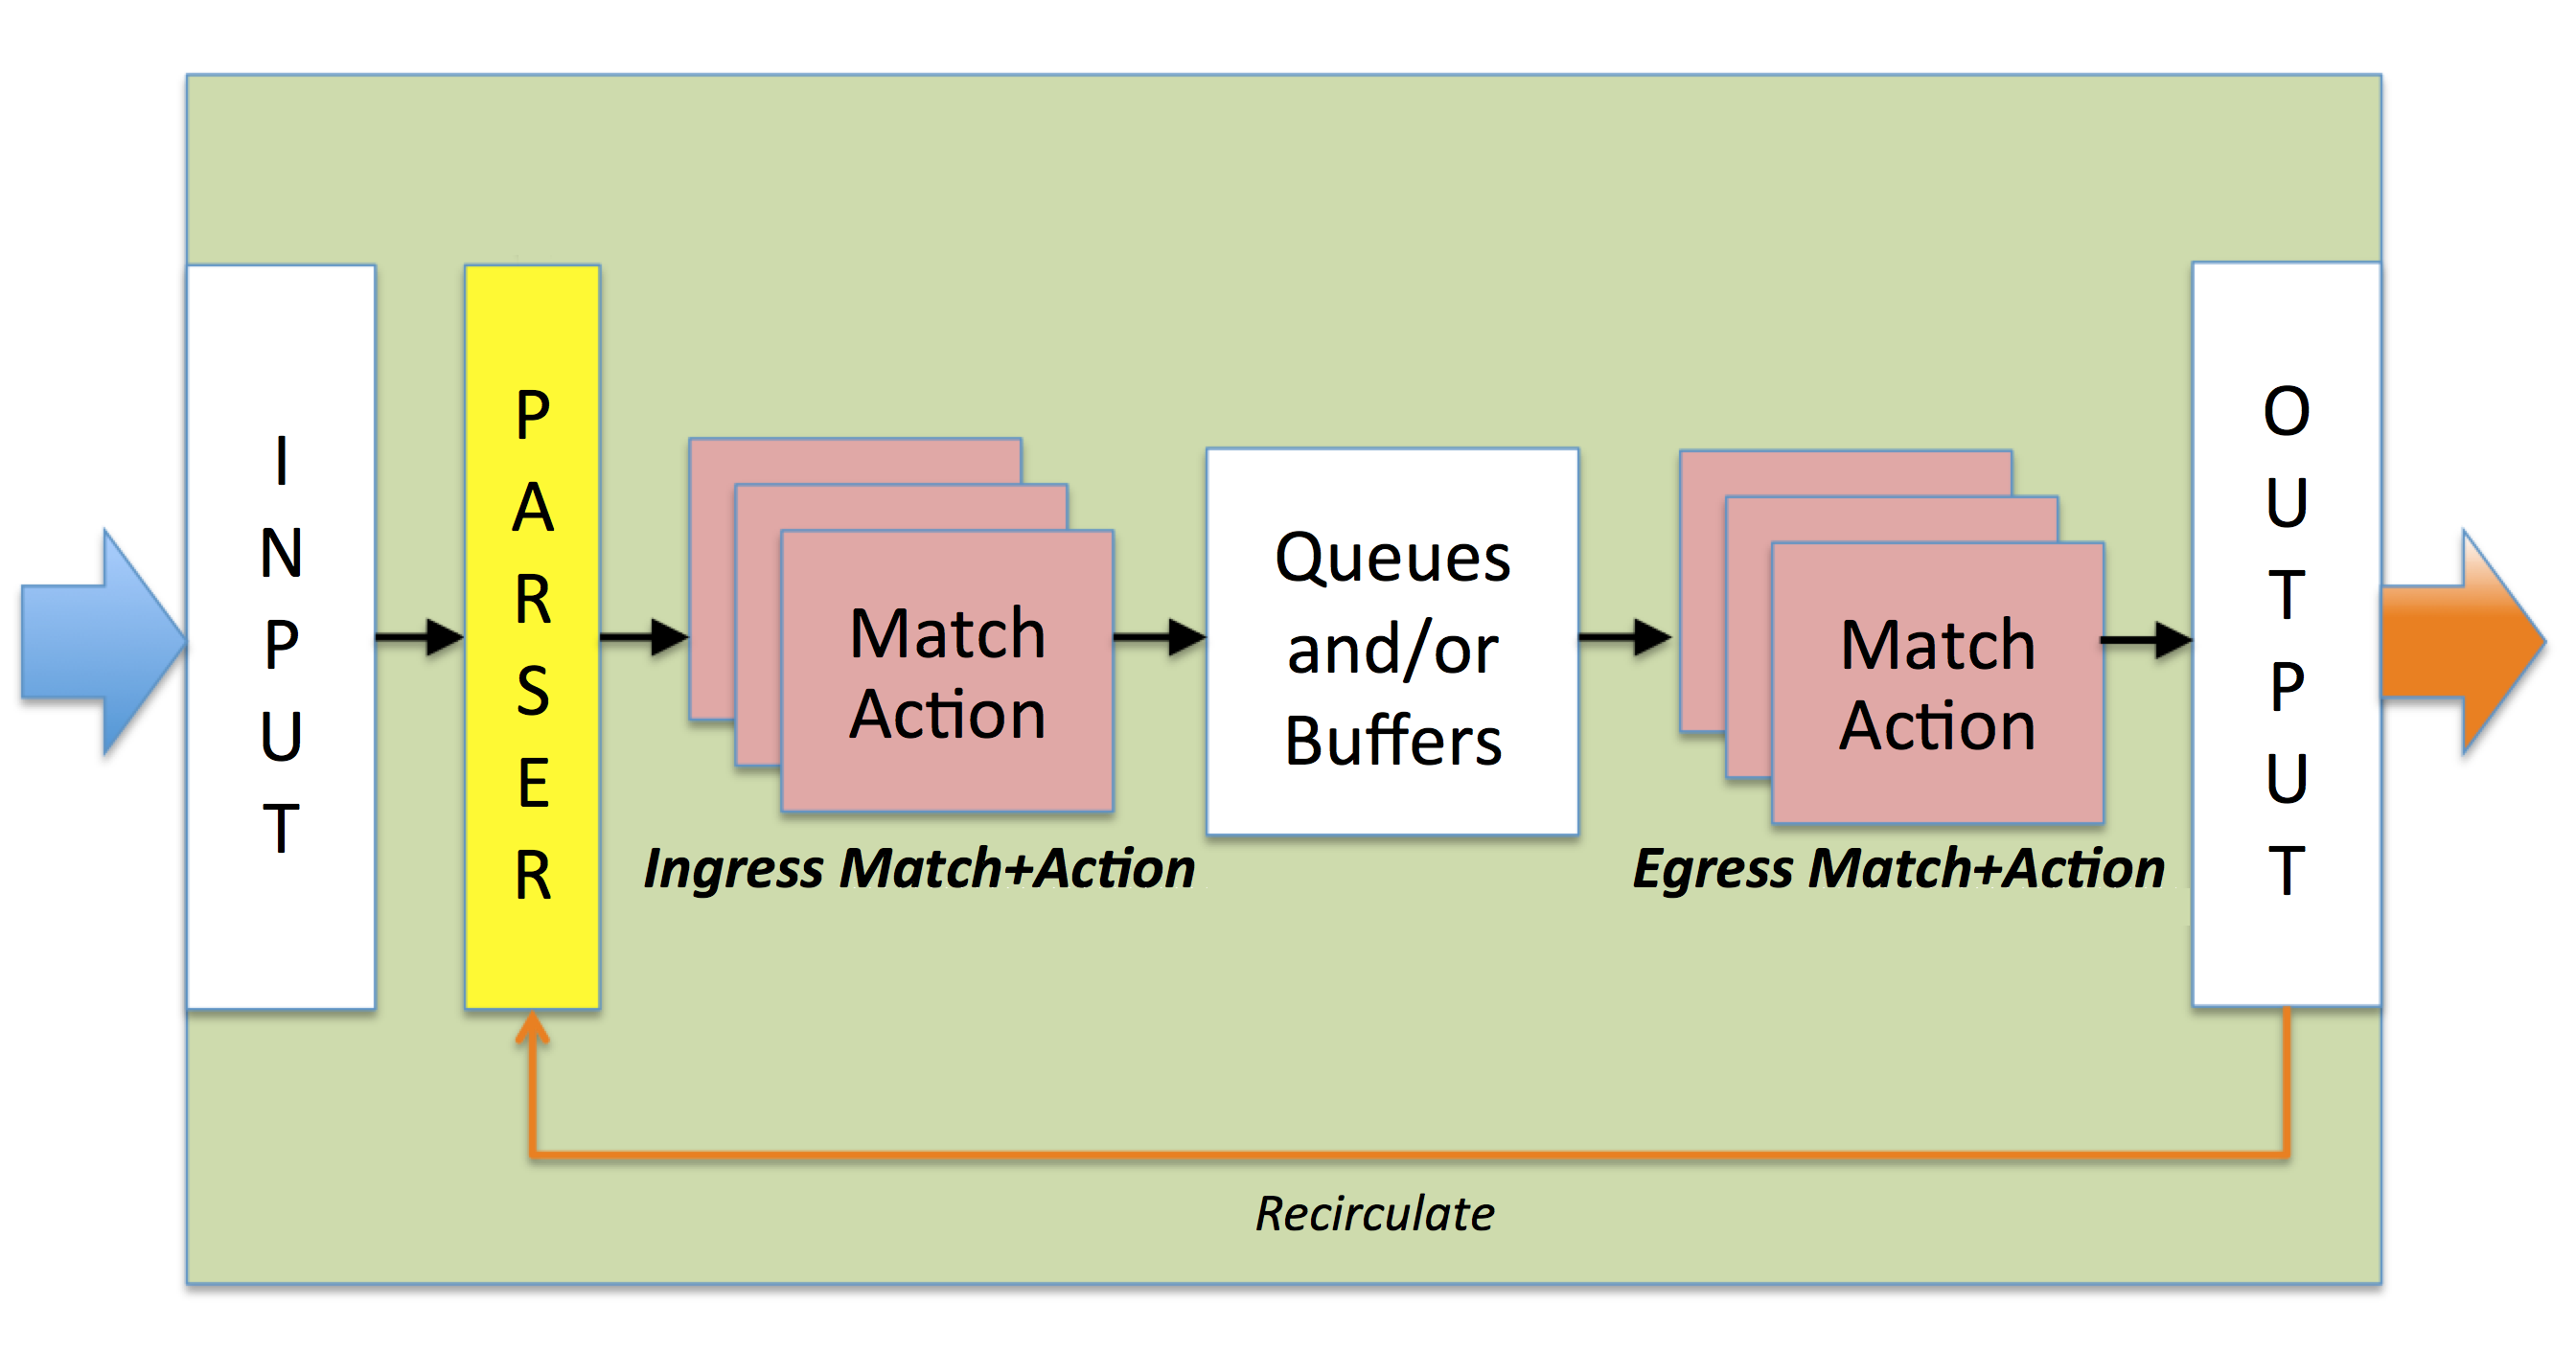
\includegraphics[width=\textwidth]{figures/recirculate.png}
    \caption{Recirculate}
    \label{fig:recirc}
\end{figure}

Figure~\ref{fig:recirc} shows the path for recirculating a packet to the parser
for processing. After the packet has completed both ingress and egress
processing, it is deparsed and sent back to the parser. The new packet is
reparsed, possibly with metadata preserved from the original packet, and passed
to the ingress pipeline as usual.

The \texttt{packet_metadata.type} metadata field distinguishes between first and
later times the packet is being processed.

Recirculation is performed by setting the 'recirculate' bit in the egress
pipeline's control metadata. The header instance pointed to by the egress
whitebox's 'recirculation_header' parameter will be appended to the
beginning of the packet, if it is valid.

\SECTION{Appendices}{append}

\SUBSECTION{Errata}{errata}

TODO

\SUBSECTION{Programming Conventions}{progconventions}

The following is a list of conventions suggested for P4 programs.

TODO

\SUBSECTION{Revision History}{revhistory}

\begin{table}[H]
\begin{center}
\begin{tabular}{| l | l | p{.6\textwidth} |} \hline
\textbf{Release} &
\textbf{Release Date} &
\textbf{Summary of Changes} \\  \hline
1.0.0-rc1 & 2014-09-08 & First public version. \\  \hline
1.0.0-rc2 & 2014-09-09 & Minor typos. \\  \hline
1.0.0-rc3 & 2014-12-30 & Fixed some missing tildes (negations). Drop in parser is now \texttt{parser_drop}. Added \texttt{add} primitive action. Added errata section. \\  \hline
1.0.1 & 2015-01-28 & Added action profiles and action selectors. Added attribute \texttt{support_timeout} to tables. \\  \hline
1.0.2 & 2015-03-03 & Added \texttt{push} and \texttt{pop} primitive actions. \\  \hline
1.1.0-rc1 & - & Added types, typed signatures, parser subroutines, blackboxes, white boxes, and local variable syntactic sugar. Separated architecture and common objects from core spec and moved into standard library. \\  \hline
\end{tabular}
\end{center}
\caption{Revision History}
\label{tab:revhistory}
\end{table}


\SUBSECTION{Terminology (Incomplete)}{terms}

\begin{table}[H]
\begin{center}
\begin{tabular}{| l | p{.7\textwidth} |} \hline
\textbf{Term} &
\textbf{Definition} \\ \hline
Control Flow &
The logic that selects which tables are applied to a packet when it is processed by a pipeline.  Used to resolve order dependencies. \\ \hline
Egress Queuing &
An abstract P4 functional block logically separating ingress and egress processing. Implementations may expose queuing and buffer resource management interfaces for this block, but this not specified by P4. \\ \hline
Egress Specification &
Metadata set by the ingress pipeline which determines the set of destination ports (and number of instances on each port) to which the packet should be sent  \\ \hline
Order Dependency &
A sequence of match and action operations whose result depends on the order of execution. For example, one table may set a field which another table uses for a match. The control flow is used to determine which of the possible effects is intended. \\ \hline
Parsed Representation &
A representation of a packet's header as a set of header instances, each of which is composed of fields. \\ \hline
Parser &
A functional block which maps a packet to a Parsed Representation \\ \hline
Pipeline &
A sequence of \matchaction tables.  \\ \hline
Run time &
When a switch is processing packets. This is distinguished from configuration time, though these operations may occur at the same time in some implementations. \\ \hline
\end{tabular}
\end{center}
\caption{Terminology}
\label{tab:terminology}
\end{table}

\SUBSECTION{Summary of P4 BNF}{bnfsummary}

%%bnf
\begin{lstlisting}[style=BNFstyle]
p4_program ::= p4_declaration +

p4_declaration ::=
    header_type_declaration | 
    header_instance_declaration |
    local_variable_declaration |
    struct_type_declaration | 
    struct_instance_declaration |
    field_list_declaration |
    parser_function_declaration |
    parser_exception_declaration |
    action_function_declaration |
    table_declaration |
    whitebox_type_declaration |
    whitebox_instance_declaration |
    whitebox_prototype_declaration |
    blackbox_type_declaration |
    blackbox_instance_declaration |
    control_function_declaration |
    typedef_declaration

const_value ::=
    bool_value |
    [ "+" | - ] [ width_spec ] unsigned_value

unsigned_value ::= 
    binary_value | 
    decimal_value | 
    hexadecimal_value

bool_value ::= true | false
binary_value ::=  binary_base binary_digit+
decimal_value ::= decimal_digit+
hexadecimal_value ::= hexadecimal_base hexadecimal_digit+

binary_base ::= 0b | 0B
hexadecimal_base ::= 0x | 0X

binary_digit ::= _ | 0 | 1
decimal_digit ::= binary_digit | 2 | 3 | 4 | 5 | 6 | 7 | 8 | 9
hexadecimal_digit ::= 
    decimal_digit | a | A | b | B | c | C | d | D | e | E | f | F

width_spec ::= decimal_digit+ :
field_value ::= const_value

type_spec ::=
    header [ header_type_name ] |
    metadata [ header_type_name ] |
    struct [ struct_type_name ] |
    blackbox [ blackbox_type_name ] |
    whitebox [ whitebox_type_name ] |
    header_array |
    field_list |
    parser |
    parser_exception |
    action |
    table |
    control |
    data_type

data_type ::=
    bit |
    bit < decimal_digit+ [ , data_type_qualifier ]* > |
    bit < auto > |
    varbit < decimal_digit+ > |
    int | 
    void

data_type_qualifier ::= signed | saturating

typedef_declaration ::=
    typedef type_spec new_type_name ;

object_ref ::=
    object_name |
    header_ref |
    field_ref |
    object_name . object_ref

general_expr ::= 
    bool_expr | arith_expr | object_ref

bool_expr ::=
    valid ( object_ref ) | bool_expr bool_op bool_expr |
    not bool_expr | ( bool_expr ) | arith_expr rel_op arith_expr |
    bool_value

arith_expr ::=
    object_ref | value | 
    max ( arith_expr , arith_expr ) | min ( arith_expr , arith_expr ) |
    ( arith_expr ) | arith_expr bin_op arith_expr | un_op arith_expr

bin_op ::= "+" | "*" | - | << | >> | & | "|" | ^
un_op ::= ~ | -
bool_op ::= or | and
rel_op ::= > | >= | == | <= | < | !=

header_type_declaration ::= 
   header_type header_type_name { header_dec_body }

header_dec_body ::=
    fields { field_dec * }
    [ length : length_exp ; ]

field_dec ::= type_spec field_name ;
length_bin_op ::= "+" | - | "*" | << | >>
length_exp ::=
    const_value |
    field_name |
    length_exp length_bin_op length_exp |
    ( length_exp )

header_instance_declaration ::=
    header header_type_name instance_name ; |
    header header_type_name instance_name "[" const_value "]" ; |
    metadata header_type_name instance_name [ metadata_initializer ] ;

metadata_initializer ::= { [ field_name : field_value ; ] + }

local_variable_declaration ::= local type_spec variable_name;

struct_type_declaration ::=
    struct_type struct_type_name { struct_member* }

struct_member ::=
    header_instance_declaration |
    struct_instance_declaration

struct_instance_declaration ::=
    struct struct_type_name instance_name ;
header_ref ::= instance_name | instance_name "[" index "]"
index ::= const_value | last | next

field_ref ::= header_ref . field_name
field_list_declaration ::=
    field_list field_list_name {
        [ field_list_entry ; ] *
    }

field_list_entry ::= 
    object_ref | field_value
parser_function_declaration ::=
    parser parser_state_name { parser_function_body }

parser_function_body ::=
    parser_body_call*
    return_statement

parser_body_call ::= 
    extract_statement |
    set_statement |
    parser_subroutine_call |
    blackbox_method_call ;

extract_statement ::= extract ( object_ref ); 

set_statement ::= set_metadata ( object_ref , metadata_expr ) ;
metadata_expr ::= field_value | field_or_data_ref

parser_subroutine_call ::= object_ref ( ) ; 

return_statement ::=
    return_value_type |
    return select ( select_exp ) { case_entry + }

return_value_type ::= 
    return object_ref ; | 
    return accept ;

case_entry ::= value_list : case_return_value_type ;
value_list ::= value_or_masked [ , value_or_masked ]* | default

case_return_value_type ::= 
    object_ref | 
    accept

value_or_masked ::=
    field_value | field_value mask field_value

select_exp ::= field_or_data_ref [, field_or_data_ref] * 
field_or_data_ref ::=
    object_ref |
    latest.field_name |
    current ( const_value , const_value )
parser_exception_declaration ::=
    parser_exception parser_exception_name {
        set_statement *
        return_or_drop ;
    }

return_or_drop ::= return_to_control | parser_drop
return_to_control ::= return control_function_name
action_function_declaration ::=
    action action_name ( [ param_list ] ) { action_statement + } |
    action action_name ( [ param_list ] ) ;

action_header ::= action_name ( [ param_list ] )

param_list ::= param [, param]*
param ::= param_qualifier* type_spec param_name

param_qualifier ::= in | out | inout | optional

action_statement ::= 
    action_name ( [ arg_list ] ) ; |
    blackbox_method_call ;

arg_list ::= general_expr [, general_expr]*


table_declaration ::=
    table table_name {
        table_attribute *
    }

table_attribute ::=
    reads { field_match * } |
    actions { [ action_name ; ] * } |
    min_size : const_value ; |
    max_size : const_value ; |
    size : const_value ; |
    modifier : blackbox_instance_name ; |
    support_timeout : bool_value ; |

field_match ::= possibly_masked_ref : field_match_type ;
possibly_masked_ref ::= 
    object_ref | object_ref mask const_value

field_match_type ::= exact | ternary | lpm | range | valid

control_function_declaration ::=
    control control_fn_name control_block
control_block ::= { control_statement * }
control_statement ::= 
    apply_call |
    apply_and_select_block |
    blackbox_method_call ; |
    if_else_statement |
    control_fn_name ( ) ; |
    return ;

apply_call ::= apply ( table_name ) ;
apply_and_select_block ::= apply ( table_name ) { [ case_list ] }
case_list ::= action_case + | hit_miss_case +
action_case ::= action_or_default control_block
action_or_default ::= action_name | default
hit_miss_case ::= hit_or_miss control_block
hit_or_miss ::= hit | miss

if_else_statement ::=
    if ( bool_expr ) control_block
    [ else_block ]

else_block ::= else control_block | else if_else_statement

whitebox_type_declaration ::= 
    whitebox_type type_name ( param_list ) { 
        p4_declaration*
    }
whitebox_instance_declaration ::= 
    whitebox type_name instance_name ( arg_list ) ;

whitebox_prototype_declaration ::= 
    whitebox_type type_name ( param_list ) ; |
    whitebox_type type_name < type_variable_list > ( param_list ) ;

type_variable_list ::= variable_name [ , variable_name ]*


blackbox_type_declaration ::= 
    blackbox_type type_name {
        member_declaration*
    }

member_declaration ::= attribute_declaration | method_declaration

method_declaration ::= 
    method method_name ( param_list );

attribute_declaration ::= 
    attribute attribute_name {
        type : attribute_type ;
        [ optional ; ]
        [ expression_local_variables : { identifier_list+ } ]
    }

identifier_list ::= variable_name ;

attribute_type ::= 
    type_spec | string | expression | block


blackbox_instance_declaration ::= 
    blackbox type_name instance_name ; |
    blackbox type_name instance_name { 
        blackbox_attribute_binding +
    }

blackbox_attribute_binding ::=
    attribute_name : object_ref ; |
    attribute_name : single_line_text ; |
    attribute_name { block_text }

blackbox_method_call ::= 
    object_ref . method_name ( arg_list )


\end{lstlisting}
%%endbnf

\SUBSECTION{P4 Reserved Words}{reservedwords}

The following are reserved words in P4 and should not be used as identifiers.\footnote{There is an open issue whether all P4 keywords will in fact be reserved.}

\begin{Verbatim}[commandchars=\\\{\}]
accept
action
and
apply
attribute
bit
blackbox
blackbox_type
block
control
current
else
expression
extract
false
field_list
fields
header
header_array
header_type
hit
if
in
inout
int
last
local
mask
max
metadata
method
min
miss
next
not
optional
or
out
parser
parser_drop
parser_exception
range
return
saturating
select
set_metadata
signed
string
struct
struct_type
table
true
typedef
valid
value
varbit
void
whitebox
whitebox_type
\end{Verbatim}

\SUBSECTION{Examples}{examples}

\SUBSUBSECTION{The Annotated mTag Example}{mtagexample}

This section presents the mTag example. The example describes two separate 
P4 programs, mtag-edge and mtag-aggregation, as described in the introduction 
in Section~\ref{sec:mtag}.

The code is written in P4 whose syntax allows the application of a C preprocessor 
to P4 files. Thus directives such as \texttt{\#define} and \texttt{\#include} are used in 
the program with the same effects as if writing C code. This is a convention 
used by these examples; the P4 language does not mandate this syntax.

The example code is split into the following files

\begin{itemize}
\item
\texttt{headers.p4}: The declaration of all header types used in both programs.
\item
\texttt{parser.p4}: The parser program shared by both programs.
\item
\texttt{actions.p4}: Common actions used by both programs.
\item
\texttt{mtag-edge.p4}: The main program for the edge switch
\item
\texttt{mtag-aggregation.p4}: The main program for any aggregation switch
\end{itemize}

The full source for all files is provided on the P4 website [2].

We start with \texttt{header.p4}. 

% For code listings: http://en.wikibooks.org/wiki/LaTeX/Source_Code_Listings

%%code
\begin{lstlisting}[style=P4style]
////////////////////////////////////////////////////////////////
// Header type definitions
////////////////////////////////////////////////////////////////

// Standard L2 Ethernet header
header_type ethernet_t {
    fields {
        bit<48> dst_addr;
        bit<48> src_addr;
        bit<16> ethertype;
    }
}

// Standard VLAN tag
header_type vlan_t {
    fields {
        bit<3>  pcp;
        bit     cfi;
        bit<12> vid;
        bit<16> ethertype;
    }
}

// The special m-tag used to control forwarding through the
// aggregation layer of  data center
header_type mTag_t {
    fields {
        bit<8>  up1;
        bit<8>  up2;
        bit<8>  down1;
        bit<8>  down2;
        bit<16> ethertype;
    }
}

// Standard IPv4 header
header_type ipv4_t {
    fields {
        bit<4> version;
        bit<4> ihl;
        bit<8> diffserv;
        bit<16> totalLen;
        bit<16> identification;
        bit<3> flags;
        bit<13> fragOffset;
        bit<8> ttl;
        bit<8> protocol;
        bit<16> hdrChecksum;
        bit<32> srcAddr;
        bit<32> dstAddr;
        varbit<320> options;
    }
    length : ihl * 4;
}


// Define a header to store global metadata - eg, metadata that
// will be shared across the ingress and egress pipelines.
header_type global_metadata_t {
    fields {
        bit     was_mtagged;   // Track if pkt was mtagged on ingr
    }
}
\end{lstlisting}
%%endcode

The parser function shared by the programs is as follows.

%%code
\begin{lstlisting}[style=P4style]
////////////////////////////////////////////////////////////////
// Parser functions and related definitions
////////////////////////////////////////////////////////////////

#import <simple_switch_architecture.h>

////////////////////////////////////////////////////////////////
//
// Header instance definitions
//
// Header instances are usually defined with the parser as
// that is where they are initialized.
//
////////////////////////////////////////////////////////////////

struct_type packet_data_t {
    header ethernet_t ethernet;
    header vlan_t vlan;
    header mTag_t mtag;
    header ipv4_t ipv4;

    metadata global_metadata_t global_metadata;    
}

////////////////////////////////////////////////////////////////
// Parser state machine description
////////////////////////////////////////////////////////////////

whitebox_type mtag_parser (
    out struct packet_data_t        p,
    in  metadata packet_metadata_t  packet_metadata
) {

    parser start {
        // Start with ethernet always.
        return p.ethernet;    
    }

    parser ethernet {
        extract(p.ethernet);
        return select(latest.ethertype) {
            0x8100:     vlan;
            0x800:      ipv4;
            default:    accept;
        }
    }

    parser vlan {
        extract(p.vlan);
        return select(latest.ethertype) {
            0xaaaa:     mtag;
            0x800:      ipv4;
            default:    accept;
        }
    }

    // mTag is allowed after a VLAN tag only
    parser mtag {
        extract(p.mtag);
        return select(latest.ethertype) {
            0x800:      ipv4;
            default:    accept;
        }
    }

    parser ipv4 {
        extract(p.ipv4);
        return accept;  // All done with parsing; start matching
    }
}
\end{lstlisting}
%%endcode

In each program, this parser whitebox will be assigned as the architecture's
parser_module using a typedef.

Here are the common actions for the two programs. The actions are defined in 
a whitebox, which will be instantiated in each program in order to hook up
the action's variables to the variables in the rest of the code.

%%code
\begin{lstlisting}[style=P4style]
////////////////////////////////////////////////////////////////
//
// actions.p4
//
// This file defines the common actions that can be exercised by
// either an edge or an aggregation switch. Since both of these
// use mostly the same actions, they are put together into 
// this file.
//
////////////////////////////////////////////////////////////////

#import <stdactions.h>
#import <simple_switch_architecture.h>

////////////////////////////////////////////////////////////////
// Actions used by tables
////////////////////////////////////////////////////////////////

whitebox_type common_actions (
    // Intrinsic metadata signals
    out bit    copy_to_cpu,
    out bit<8> cpu_code,
    out bit    drop,

    out bit<4> port_type,
    out bit    error
) {
    // Copy the packet to the CPU;
    action copy_pkt_to_cpu(in bit<8> new_cpu_code) {
        modify_field(copy_to_cpu, 1);
        modify_field(cpu_code, new_cpu_code);
    }

    // Drop the packet; optionally send to CPU
    action drop_pkt(in bit do_copy, in bit<8> new_cpu_code) {
        modify_field(copy_to_cpu, do_copy);
        modify_field(cpu_code, new_cpu_code);
        modify_field(drop, 1);
    }

    // Set the port type; see mtag_port_type. Allow error indication.
    action set_port_type(in bit<4> new_port_type, in bit new_error) {
        modify_field(port_type, new_port_type);
        modify_field(error, new_error);
    }    
}

\end{lstlisting}
%%endcode

Here is the edge program.

%%code
\begin{lstlisting}[style=P4style]
////////////////////////////////////////////////////////////////
//
// mtag-edge.p4
//
// This file defines the behavior of the edge switch in an mTag
// example.
//
// The switch is programmed to do local forwarding to a set of
// ports as well as to allow traffic between the local ports
// and a set of uplinks.  Packets on the uplink port are given
// an mTag between the VLAN and IP headers.  Locally switched
// packets should not be mTagged. The program also enforces
// that switching is not allowed between uplink ports.
//
////////////////////////////////////////////////////////////////

#import <stdactions.h>
#import <simple_switch_architecture.h>

// Include the header definitions and parser (with header instances)
#include "headers.p4"
#include "parser.p4"
#include "actions.p4"  // For actions common between edge and agg

#define PORT_COUNT 64  // Total ports in the switch

// Use the common mtag parser as our main parser module
typedef mtag_parser parser_module;

whitebox_type ingress_module (
    inout struct packet_data_t             p,
    in    metadata packet_metadata_t       packet_metadata,
    in    metadata parser_status_t         parser_status,
    out   metadata ingress_pipe_controls_t control_data,
) {

    // Local metadata declarations
    local bit<4>  port_type;     // Type of port: up, down, local...
    local bit     error;         // An error in ingress port check

    // Import actions common between edge and aggregation programs
    whitebox common_actions common (
        control_data.copy_to_cpu,
        control_data.cpu_code,
        control_data.drop,

        locals.port_type,
        locals.error
    );

    // Remove the mtag for local processing/switching
    action _strip_mtag() {
        // Strip the tag from the packet...
        remove_header(p.mtag);
        // but keep state that it was mtagged.
        modify_field(p.global_metadata.was_mtagged, 1);
    }

    // Always strip the mtag if present on the edge switch
    table strip_mtag {
        reads {
            p.mtag     : valid; // Was mtag parsed?
        }
        actions {
            _strip_mtag;        // Strip mtag and record metadata
            no_op;              // Pass thru otherwise
        }
    }

    ////////////////////////////////////////////////////////////////

    // Identify ingress port: local, up1, up2, down1, down2
    table identify_port {
        reads {
            packet_metadata.ingress_port : exact;
        }
        actions { // Each table entry specifies *one* action
            common.set_port_type;
            common.drop_pkt;        // If unknown port
            no_op;         // Allow packet to continue
        }
        max_size : PORT_COUNT; // One rule per port
    }

    // Action to set the egress port; used for local switching
    action set_egress(in bit<16> egress_spec) {
        modify_field(control_data.egress_spec, egress_spec);
    }

    // Check for "local" switching (not to aggregation layer)
    table local_switching {
        reads {
            p.vlan.vid             : exact;
            p.ipv4.dstAddr         : exact;
        }
        actions {
            set_egress;     // If switched, set egress
            no_op;
        }
    }

    // Add an mTag to the packet; select egress spec based on up1
    action add_mTag(in bit<8> up1, in bit<8> up2,
                    in bit<8> down1, in bit<8> down2)
    {
        add_header(p.mtag);
        // Copy VLAN ethertype to mTag
        modify_field(p.mtag.ethertype, p.vlan.ethertype);

        // Set VLAN's ethertype to signal mTag
        modify_field(p.vlan.ethertype, 0xaaaa);

        // Add the tag source routing information
        modify_field(p.mtag.up1, up1);
        modify_field(p.mtag.up2, up2);
        modify_field(p.mtag.down1, down1);
        modify_field(p.mtag.down2, down2);

        // Set the destination egress port as well from the tag info
        modify_field(control_data.egress_spec, up1);
    }

    // Count packets and bytes by mtag instance added
    blackbox counter pkts_by_dest {
        type : packets;
        direct : mTag_table;
    }

    blackbox counter bytes_by_dest {
        type : bytes;
        direct : mTag_table;
    }

    // Check if the packet needs an mtag and add one if it does.
    table mTag_table {
        reads {
            p.ethernet.dst_addr    : exact;
            p.vlan.vid             : exact;
        }
        actions {
            add_mTag;  // Action called if pkt needs an mtag.
            common.copy_pkt_to_cpu; // Option: If no mtag setup, 
                                      // forward to the CPU
            no_op;
        }
        max_size                 : 20000;
    }

    // The ingress control function
    control main {

        // Always strip mtag if present, save state
        apply(strip_mtag);

        // Identify the source port type
        apply(identify_port);

        // If no error from source_check, continue
        if (locals.error == 0) {
            // Attempt to switch to end hosts
            apply(local_switching);

            // If not locally switched, try to setup mtag
            if (control_data.egress_spec == 0) {
                apply(mTag_table);
            }
         }
    }
}



whitebox_type egress_module (
    inout struct packet_data_t             p,
    in    metadata packet_metadata_t       packet_metadata,
    in    metadata egress_aux_metadata_t   aux_metadata,
    out   metadata egress_pipe_controls_t  control_data,
) {

    // Local metadata declarations
    local bit<4>  port_type;     // Unused in egress
    local bit     error;         // Unused in egress

    local bit<8>  color;         // For metering

    // Import actions common between edge and aggregation programs
    whitebox common_actions common (
        control_data.copy_to_cpu,
        control_data.cpu_code,
        control_data.drop,

        locals.port_type,
        locals.error
    );

    // Packets from agg layer must stay local; enforce that here
    table egress_check {
        reads {
            packet_metadata.ingress_port : exact;
            p.global_metadata.was_mtagged : exact;
        }

        actions {    
            common.drop_pkt;
            no_op;
        }
        max_size : PORT_COUNT; // At most one rule per port
    }

    // Egress metering; this could be direct, but we let SW 
    // use whatever mapping it might like to associate the
    // meter cell with the source/dest pair
    blackbox meter per_dest_by_source {
        type : bytes;

        // One cell per source/dest pair
        instance_count : PORT_COUNT * PORT_COUNT; 
    }

    action meter_pkt(in int meter_idx) {
        per_dest_by_source.execute(locals.color, meter_idx);
    }

    // Mark packet color, for uplink ports only
    table egress_meter {
        reads {
            packet_metadata.ingress_port : exact;
            p.mtag.up1 : exact;
        }
        actions {
            meter_pkt;
            no_op;
        }
        size : PORT_COUNT * PORT_COUNT;  // Could be smaller
    }

    // Apply meter policy
    blackbox counter per_color_drops {
        type : packets;
        direct : meter_policy;
    }

    table meter_policy {
        reads {
            locals.color : exact;
        }
        actions {
            drop; // Automatically counted by direct counter above
            no_op;
        }
    }

    // The egress control function
    control main {
        // Check for unknown egress state or bad retagging with mTag.
        apply(egress_check);

        // Apply egress_meter table; if hit, apply meter policy
        apply(egress_meter) {
            hit {
                apply(meter_policy);
            }
        }
    }

}
\end{lstlisting}
%%endcode

Here is the aggregation program.

%%code
\begin{lstlisting}[style=P4style]
////////////////////////////////////////////////////////////////
//
// mtag-aggregation.p4
//
// This file defines the behavior of the aggregation switch in an
// mTag example.
//
// The switch is programmed to do forwarding strictly based
// on the mTag header. Recall there are two layers of aggregation
// in this example. Both layers use the same program. It is up
// to the application layer to determine where in the
// aggregation layer the switch is.
//
////////////////////////////////////////////////////////////////

#import <stdactions.h>
#import <simple_switch_architecture.h>

// Include the header definitions and parser (with header instances)
#include "headers.p4"
#include "parser.p4"
#include "actions.p4"  // For actions common between edge and agg

// Use the common mtag parser as our main parser module
typedef mtag_parser parser_module;

whitebox_type ingress_module (
    inout struct packet_data_t             p,
    in    metadata packet_metadata_t       packet_metadata,
    in    metadata parser_status_t         parser_status,
    out   metadata ingress_pipe_controls_t control_data,
) {
    
    // Local metadata declarations
    local bit<4>  port_type;     // Type of port: up, down, local...
    local bit     error;         // Unused in aggregation program

    // Import actions common between edge and aggregation programs
    whitebox common_actions common (
        control_data.copy_to_cpu,
        control_data.cpu_code,
        control_data.drop,

        locals.port_type,
        locals.error
    );

    ////////////////////////////////////////////////////////////////

    // Want all packets to have mTag; Apply drop or to-cpu policy
    // otherwise.
    // Will be statically programmed with one entry.
    table check_mtag {
        reads {
            p.mtag : valid; // Was mtag parsed?
        }
        actions { // Each table entry specifies *one* action
            common.drop_pkt;           // Deny if policy is to drop
            common.copy_pkt_to_cpu;    // Deny if policy is to go to CPU
            no_op;                     // Accept action
        }
        size : 1;
    }

    ////////////////////////////////////////////////////////////////

    // Identify ingress port: local, up1, up2, down1, down2
    table identify_port {
        reads {
            packet_metadata.ingress_port : exact;
        }
        actions { // Each table entry specifies *one* action
            common.set_port_type;
            common.drop_pkt;        // If unknown port
            no_op;       // Allow packet to continue
        }
        max_size : 64; // One rule per port
    }

    ////////////////////////////////////////////////////////////////

    // Actions to copy the proper field from mtag into the egress spec
    action use_mtag_up1() {
        // This is actually never used on agg switches
        modify_field(control_data.egress_spec, p.mtag.up1);
    }
    action use_mtag_up2() {
        modify_field(control_data.egress_spec, p.mtag.up2);
    }
    action use_mtag_down1() {
        modify_field(control_data.egress_spec, p.mtag.down1);
    }
    action use_mtag_down2() {
        modify_field(control_data.egress_spec, p.mtag.down2);
    }

    // Table to select output spec from mtag
    table select_output_port {
        reads {
            locals.port_type  : exact; // Up or down, level 1 or 2.
        }
        actions {
            use_mtag_up1;
            use_mtag_up2;
            use_mtag_down1;
            use_mtag_down2;

            // If port type is not recognized, apply previous policy:
            no_op; 
        }
        max_size : 4; // Only need one entry per port type
    }

    // The ingress control function
    control main {
        // Verify mTag state and port are consistent
        apply(check_mtag);
        apply(identify_port);
        apply(select_output_port);
    }
}

whitebox_type egress_module (
    inout struct packet_data_t             p,
    in    metadata packet_metadata_t       packet_metadata,
    in    metadata egress_aux_metadata_t   aux_metadata,
    out   metadata egress_pipe_controls_t  control_data,
) {
    // No egress functionality needed for this example.
    control main { }
}
\end{lstlisting}
%%endcode

The following is an example C header file that might be used with the mtag
example above. This shows the following:

\begin{itemize}
\item
Type definitions for port types (\texttt{mtag_port_type_t}) meter levels \\
(\texttt{mtag_meter_levels_t}) 
and a table entry handle (\texttt{entry_handle_t}).  
\item
An example function to add an entry to the \texttt{identify_port} table, \\
\texttt{table_identify_port_add_with_set_port_type}. 
The action to use with the entry is indicated at the end of the function name: 
\texttt{set_port_type}.
\item
Functions to set the default action for the identify_port table: \\
\texttt{table_indentify_port_default_common_drop_pkt} and \\
\texttt{table_indentify_port_default_common_set_port_type}.
\item
A function to add an entry to the mTag table: \\
\texttt{table_mTag_table_add_with_add_mTag}
\item
A function to get a counter associated with the meter table: \\
\texttt{counter_per_color_drops_get}.
\end{itemize}

\begin{lstlisting}[language=C,frame=single,backgroundcolor=\color{nonp4orange}]
/**
 * Run time header file example for CCR mTag example
 */


#ifndef MTAG_RUN_TIME_H
#define MTAG_RUN_TIME_H

/**
 * @brief Port types required for the mtag example
 *
 * Indicates the port types for both edge and aggregation
 * switches.
 */

typedef enum mtag_port_type_e {
    MTAG_PORT_UNKNOWN,        /* Uninitialized port type */
    MTAG_PORT_LOCAL,          /* Locally switch port for edge */
    MTAG_PORT_EDGE_TO_AG1,    /* Up1: edge to agg layer 1 */
    MTAG_PORT_AG1_TO_AG2,     /* Up2: Agg layer 1 to agg layer 2 */
    MTAG_PORT_AG2_TO_AG1,     /* Down2: Agg layer 2 to agg layer 1 */
    MTAG_PORT_AG1_TO_EDGE,     /* Down1: Agg layer 1 to edge */
    MTAG_PORT_ILLEGAL,        /* Illegal value */
    MTAG_PORT_COUNT
} mtag_port_type_t;

/**
 * @brief Colors for metering
 *
 * The edge switch supports metering from local ports up to the
 * aggregation layer.
 */

typedef enum mtag_meter_levels_e {
    MTAG_METER_COLOR_GREEN,  /* No congestion indicated */
    MTAG_METER_COLOR_YELLOW, /* Above low water mark */
    MTAG_METER_COLOR_RED,    /* Above high water mark */
    MTAG_METER_COUNT
} mtag_meter_levels_t;

typedef uint32_t entry_handle_t;

/* mTag table */

/**
 * @brief Add an entry to the edge identify port table
 * @param ingress_port The port number being identified
 * @param port_type The port type associated with the port
 * @param ingress_error The value to use for the error indication
 */

entry_handle_t table_identify_port_add_with_set_port_type(
    uint32_t ingress_port, 
    mtag_port_type_t port_type,
    uint8_t ingress_error);

/**
 * @brief Set the default action of the identify port
 * table to send the packet to the CPU.
 * @param do_copy Set to 1 if should send copy to the CPU
 * @param cpu_code If do_copy, this is the code used
 * @param bad_packet Set to 1 to flag packet as bad
 *
 * This allows the programmer to say: If port type is not
 * set, this is an error; let me see the packet.
 *
 * Also allows just a drop of the packet.
 */

int table_indentify_port_default_common_drop_pkt(
    uint8_t do_copy,
    uint16_t cpu_code,
    uint8_t bad_packet);

/**
 * @brief Set the default action of the identify port
 * table to set to the given value
 * @param port_type The port type associated with the port
 * @param ingress_error The value to use for the error indication
 *
 * This allows the programmer to say "default port type is local"
 */

int table_indentify_port_default_common_set_port_type(
    mtag_port_type_t port_type,
    uint8_t ingress_error);

/**
 * @brief Add an entry to the add mtag table
 * @param dst_addr The L2 destination MAC for matching
 * @param vid The VLAN ID used for matching
 * @param up1 The up1 value to use in the mTag
 * @param up2 The up2 value to use in the mTag
 * @param down1 The down1 value to use in the mTag
 * @param down2 The down2 value to use in the mTag
 */
entry_handle_t table_mTag_table_add_with_add_mTag(
    mac_addr_t dst_addr, uint16_t vid,
    uint8_t up1, uint8_t up2, uint8_t down1, uint8_t down2);

/**
 * @brief Get the number of drops by ingress port and color
 * @param ingress_port The ingress port being queried.
 * @param color The color being queried.
 * @param count (output) The current value of the parameter.
 * @returns 0 on success.
 */
int counter_per_color_drops_get(
    uint32_t ingress_port,
    mtag_meter_levels_t color,
    uint64_t *count);

#endif /* MTAG_RUN_TIME_H */
\end{lstlisting}

\SUBSUBSECTION{Adding Hysteresis to mTag Metering with Registers}{hysteresis}

In the previous section, the mtag-edge switch used metering between local 
ports and the aggregation layer. Suppose that network simulation indicated 
a benefit if hysteresis could be used with the meters. That is, once the meter 
was red, packets are discarded until the meter returned to green (not just 
to yellow).
This can be achieved by adding a register set parallel to the meters. Each 
cell in the register set holds the "previous" color of the meter. 

Here is the updated edge program to support this feature. The meter index is
stored in local metadata for convenience.

%%code
\begin{lstlisting}[style=P4style]
////////////////////////////////////////////////////////////////
//
// mtag-edge.p4
//
// This file defines the behavior of the edge switch in an mTag
// example.
//
// The switch is programmed to do local forwarding to a set of
// ports as well as to allow traffic between the local ports
// and a set of uplinks.  Packets on the uplink port are given
// an mTag between the VLAN and IP headers.  Locally switched
// packets should not be mTagged. The program also enforces
// that switching is not allowed between uplink ports.
//
////////////////////////////////////////////////////////////////

#import <stdactions.h>
#import <simple_switch_architecture.h>

// Include the header definitions and parser (with header instances)
#include "headers.p4"
#include "parser.p4"
#include "actions.p4"  // For actions common between edge and agg

#define PORT_COUNT 64  // Total ports in the switch

// Use the common mtag parser as our main parser module
typedef mtag_parser parser_module;

whitebox_type ingress_module (
    inout struct packet_data_t             p,
    in    metadata packet_metadata_t       packet_metadata,
    in    metadata parser_status_t         parser_status,
    out   metadata ingress_pipe_controls_t control_data,
) {

    // Local metadata declarations
    local bit<4>  port_type;     // Type of port: up, down, local...
    local bit     error;         // An error in ingress port check

    // Import actions common between edge and aggregation programs
    whitebox common_actions common (
        control_data.copy_to_cpu,
        control_data.cpu_code,
        control_data.drop,

        locals.port_type,
        locals.error
    );

    // Remove the mtag for local processing/switching
    action _strip_mtag() {
        // Strip the tag from the packet...
        remove_header(p.mtag);
        // but keep state that it was mtagged.
        modify_field(p.global_metadata.was_mtagged, 1);
    }

    // Always strip the mtag if present on the edge switch
    table strip_mtag {
        reads {
            p.mtag     : valid; // Was mtag parsed?
        }
        actions {
            _strip_mtag;        // Strip mtag and record metadata
            no_op;              // Pass thru otherwise
        }
    }

    ////////////////////////////////////////////////////////////////

    // Identify ingress port: local, up1, up2, down1, down2
    table identify_port {
        reads {
            packet_metadata.ingress_port : exact;
        }
        actions { // Each table entry specifies *one* action
            common.set_port_type;
            common.drop_pkt;        // If unknown port
            no_op;         // Allow packet to continue
        }
        max_size : PORT_COUNT; // One rule per port
    }

    // Action to set the egress port; used for local switching
    action set_egress(in bit<16> egress_spec) {
        modify_field(control_data.egress_spec, egress_spec);
    }

    // Check for "local" switching (not to aggregation layer)
    table local_switching {
        reads {
            p.vlan.vid             : exact;
            p.ipv4.dstAddr         : exact;
        }
        actions {
            set_egress;     // If switched, set egress
            no_op;
        }
    }

    // Add an mTag to the packet; select egress spec based on up1
    action add_mTag(in bit<8> up1, in bit<8> up2,
                    in bit<8> down1, in bit<8> down2)
    {
        add_header(p.mtag);
        // Copy VLAN ethertype to mTag
        modify_field(p.mtag.ethertype, p.vlan.ethertype);

        // Set VLAN's ethertype to signal mTag
        modify_field(p.vlan.ethertype, 0xaaaa);

        // Add the tag source routing information
        modify_field(p.mtag.up1, up1);
        modify_field(p.mtag.up2, up2);
        modify_field(p.mtag.down1, down1);
        modify_field(p.mtag.down2, down2);

        // Set the destination egress port as well from the
        // tag info
        modify_field(control_data.egress_spec, up1);
    }

    // Count packets and bytes by mtag instance added
    blackbox counter pkts_by_dest {
        type : packets;
        direct : mTag_table;
    }

    blackbox counter bytes_by_dest {
        type : bytes;
        direct : mTag_table;
    }

    // Check if the packet needs an mtag and add one if it does.
    table mTag_table {
        reads {
            p.ethernet.dst_addr    : exact;
            p.vlan.vid             : exact;
        }
        actions {
            // Action called if pkt needs an mtag:
            add_mTag; 

            // Option: If no mtag setup, forward to the CPU
            common.copy_pkt_to_cpu; 

            no_op;
        }
        max_size                 : 20000;
    }

    // The ingress control function
    control main {

        // Always strip mtag if present, save state
        apply(strip_mtag);

        // Identify the source port type
        apply(identify_port);

        // If no error from source_check, continue
        if (locals.error == 0) {
            // Attempt to switch to end hosts
            apply(local_switching);

            // If not locally switched, try to setup mtag
            if (control_data.egress_spec == 0) {
                apply(mTag_table);
            }
         }
    }
}



whitebox_type egress_module (
    inout struct packet_data_t             p,
    in    metadata packet_metadata_t       packet_metadata,
    in    metadata egress_aux_metadata_t   aux_metadata,
    out   metadata egress_pipe_controls_t  control_data,
) {


    // Local metadata declarations
    local bit<4>  port_type;     // Unused in egress
    local bit     error;         // Unused in egress

    local bit<8>  color;         // For metering
    local bit<8> prev_color;     // For metering
    local bit<32> meter_idx;

    // Import actions common between edge and aggregation programs
    whitebox common_actions common (
        control_data.copy_to_cpu,
        control_data.cpu_code,
        control_data.drop,

        locals.port_type,
        locals.error
    );

    // Packets from agg layer must stay local; enforce that here
    table egress_check {
        reads {
            packet_metadata.ingress_port : exact;
            p.global_metadata.was_mtagged : exact;
        }

        actions {    
            common.drop_pkt;
            no_op;
        }
        max_size : PORT_COUNT; // At most one rule per port
    }

    // Egress metering; this could be direct, but we let SW 
    // use whatever mapping it might like to associate the
    // meter cell with the source/dest pair
    blackbox meter per_dest_by_source {
        type : bytes;

        // One cell per source/dest pair
        instance_count : PORT_COUNT * PORT_COUNT;
    }

    // This function updated to track meter index and prev color register
    action meter_pkt(in int meter_idx) {
        // Save index and previous color in metadata; see below.
        modify_field(locals.meter_idx, meter_idx);
        prev_color_per_port.get(locals.prev_color, meter_idx);
        per_dest_by_source.execute(locals.color, meter_idx);
    }

    // Mark packet color, for uplink ports only
    table egress_meter {
        reads {
            packet_metadata.ingress_port : exact;
            p.mtag.up1 : exact;
        }
        actions {
            meter_pkt;
            no_op;
        }
        size : PORT_COUNT * PORT_COUNT;  // Could be smaller
    }

    ////////////////////////////////////////////////////////////////
    // Support added for hysteresis on the meter
    //
    // Keep the meter's old state in a register. Update the register
    // only on transtions => red or => green. Override the meter 
    // decision if the register indicates the state was red.
    //
    ////////////////////////////////////////////////////////////////

    // The register stores the "previous" state of the color.
    // Index is the same as that used by the meter.
    blackbox register prev_color_per_port {
        width : 8;

        // Paired with the meters above:
        instance_count : PORT_COUNT * PORT_COUNT;
    }

    // Action: Update the color saved in the register
    action update_prev_color(in bit<8> new_color) {
        prev_color_per_port.set(new_color, locals.meter_idx);
    }

    // Action: Override packet color with that from the parameter
    action mark_pkt(in bit<8> color) {
        modify_field(locals.color, color);
    }

    //
    // This table is statically populated with the following rules:
    //   color: green,  prev_color: red   ==> update_prev_color(green)
    //   color: red,    prev_color: green ==> update_prev_color(red)
    //   color: yellow, prev_color: red   ==> mark_pkt(red)
    // Otherwise, no-op.

    table hysteresis_check {
        reads {
            locals.color : exact;
            locals.prev_color : exact;
        }
        actions {
            update_prev_color;
            mark_pkt;
            no_op;
        }
        size : 4;
    }

    // Apply meter policy
    blackbox counter per_color_drops {
        type : packets;
        direct : meter_policy;
    }

    // Apply meter policy to the packet based on its color
    table meter_policy {
        reads {
            locals.color : exact;
        }
        actions {
            drop; // Automatically counted by direct counter above
            no_op;
        }
    }

    // The egress control function
    control main {
        // Check for unknown egress state or bad retagging with mTag.
        apply(egress_check);

        // Apply egress_meter table; if hit, apply meter policy
        apply(egress_meter) {
            hit {
                apply(hysteresis_check);
                apply(meter_policy);
            }
        }
    }

}
\end{lstlisting}
%%endcode


\SUBSUBSECTION{ECMP Selection Example}{ecmpselection}

This example shows how ECMP can be implemented using table modifiers.

%%code
\begin{lstlisting}[style=P4style]
table ipv4_routing {
    reads {
        ipv4.dstAddr: lpm;
    }
    actions {
        nhop_set;
        no_op;
    }
    modifier : ecmp_action_profile;
    size : 16384;    // 16K possible IPv4 prefixes
}

blackbox action_profile ecmp_action_profile {
    size : 4096;    // 4K possible next hops
    dynamic_action_selection : ecmp_hash;
}

// list of fields used to determine the ECMP next hop
field_list l3_hash_fields {
    ipv4.srcAddr;
    ipv4.dstAddr;
    ipv4.protocol;
    ipv4.protocol;
    tcp.sport;
    tcp.dport;
}

blackbox hash_calculation ecmp_hash {
    input {
        l3_hash_fields;
    }
    algorithm : crc16;
    output_width : 16;
}

\end{lstlisting}
%%endcode


\SUBSECTION{Feature Proposals for Future Versions}{featureproposals}

P4 is expected to evolve and develop as its features are exercised and issues 
are found. Incremental improvements will be released with minor version number 
updates. This section lists features under consideration for coming P4 versions.


\begin{table}[H]
\begin{center}
\begin{tabular}{| p{.4\textwidth} | p{.6\textwidth} |} \hline
\textbf{Title} &
\textbf{Summary} \\ \hline
Enum types &
Allow declaration and comparison of enum types similar to that of C
or Java \\ \hline
Support Assignment Operators &
Allow fields and headers to be manipulated with assignment operators 
such as = or +=. \\ \hline
Better Encapsulation Support &
Support better action primitives and parsing functionality for encapsulation 
applications. \\ \hline
Run Time Reconfiguration &
Consider language features and conventions that would better enable consistent 
run time reconfigurability. \\ \hline
Field and Header Aliasing &
Support a mechanism allowing references to different field or header instances 
via indirection (an alias) to allow the application of policy across multiple 
packet formats simultaneously.  \\ \hline
Flexible feature inclusion &
Add facilities allowing compile or run time selection of features based on 
availability. \\ \hline
Debugging Features &
Support better debuggability with the addition of features such as object 
introspection, variable logging levels and event triggering. \\ \hline
Indirect Table Matching &
Support database-like tables which can be queried multiple times by \matchaction. \\ \hline
\end{tabular}
\end{center}
\caption{Feature Proposals}
\label{tab:featureprops}
\end{table}

\SUBSECTION{References}{references}

[1] Bosshart, et al. \textit{P4: Programming Protocol-Independent Packet Processors}. 
Computer Communication Review, July 2014.  \url{http://www.sigcomm.org/ccr/papers/2014/July/0000000.0000004}.

[2] The P4 Language Consortium web site. \url{http://www.p4.org}.

\end{document}
